\chapter{Introducción}
Analizar y cuantificar todo un inventario forestal puede tomar mucho tiempo, puede tender a fallar por una u otra razón, por lo que la falla humana está presente en todo momento, más sin embargo, las tecnologías que hoy en día se han desarrollado además de distintos ámbitos de la ciencia pueden ayudar a automatizar tareas y reducir el índice de error humano.

El \emph{aprendizaje máquina}\footnote{Campo de la inteligencia artificial que desarrolla algoritmos capaces de aprender por medio de información.} es precisamente uno de los campos de la \emph{inteligencia artificial}\footnote{Ciencia encargada de desarrollar algoritmos capaces de imitar capacidades humanas.} que permite resolver esta clase de problemas, ya que gracias al aprendizaje supervisado se pueden usar técnicas de agrupamiento para clasificar distintas especies de árboles por medio de muestras recolectadas. En el caso del análisis de recorridos por drones, el enfoque está dirigido al área forestal dado que se puede utilizar el aprendizaje máquina para la gestión del inventario forestal, ayudando a reducir el fallo humano y optimizando las tareas de clasificación de especies arbóreas.

Para llevar a cabo la tarea de clasificar las especies arbóreas, se recolectaron muestras de las zonas del Cilantrillo y La Trinidad en Nuevo León. Estas zonas cuentan con distintas zonas especies arbóreas como lo son: \emph{Abies, Encino y Pino}.
\newpage

\vspace*{3\baselineskip}

En las figura \ref{Zona-trinidad} se aprecia la zona de Trinidad desde distintas alturas en el mapa, el rectángulo azúl en la figura es la zona sobre la que se hizo el recorrido.

\begin{figure}[h!]
  \centering
\begin{tabular}{@{}ccc@{}}
\subfloat[Estatal]{\includegraphics[width=0.3\textwidth]{Lejos_t}} & 
\subfloat[Municipal]{\includegraphics[width=0.3\textwidth]{Medio_t}} &
\subfloat[Local]{\includegraphics[width=0.3\textwidth]{Cerca_t}}
  \end{tabular}
  \caption[Mapa de Trinidad.]{La Trinidad, Santiago, Nuevo León (25.225939, -100.1431609).}
  \label{Zona-trinidad}
\end{figure}

\hspace{15 cm}

En las figura \ref{Zona-cilantrillo} se aprecia la zona de Trinidad desde distintas alturas en el mapa, el rectángulo azúl en la figura es la zona sobre la que se hizo el recorrido.

\begin{figure}[h!]
  \centering
\begin{tabular}{@{}ccc@{}}
\subfloat[Estatal]{\includegraphics[width=0.3\textwidth]{Lejos_C}} & 
\subfloat[Municipal]{\includegraphics[width=0.3\textwidth]{Medio_C}} &
\subfloat[Local]{\includegraphics[width=0.3\textwidth]{Cerca_C}}
  \end{tabular}
  \caption[Mapa de Cilantrillo]{El Cilantrillo, Montemorelos, Nuevo León (25.3523418, -100.3463186).}
   \label{Zona-cilantrillo}
\end{figure}

\newpage

\section{Motivación}
Pese a que ya existen mecanismos de detección de objetos, muchos de ellos no funcionan con la precisión o la meta que deseamos, puesto que no se enfocan en un objetivo en particular, más sin embargo, la investigación se enfocas puramente en la detección de especies arbóreas utilizando muestras recolectadas en las zonas del Cilantrillo y Trinidad.

\section{Hipótesis}
Se sabe que el procesamiento de imágenes tiene como finalidad enfocarse en la búsqueda de un elemento en particular, las especies arbóreas (caso del presente trabajo) se plantea demostrar que el procesamiento de imágenes permitiría reducir tiempos de recorrido a pie y optimizar costos en cuanto a la realización de inventarios forestales por medio de técnicas tradicionales.

\section{Objetivos}
En esta sección se establece el objetivo general y los objetivos específicos sobre los que se enfoca la tesis.

\subsection{Objetivo general}
El objetivo de realizar el inventario forestal por medio del procesamiento de
imágenes tiene un propósito más práctico que técnico. El algoritmo permitiría a quienes se encarguen de analizar las zonas forestales, reducir el tiempo invertido en aplicar técnicas tradicionales por técnicas de procesamiento de imágenes.

Estas técnicas  basadas en el aprendizaje máquina, el cual permitir
generar un inventario forestal mediante el recorrido de un dron y a su vez, analizarlo por medio de la inteligencia artificial con la finalidad de indicar las cantidad de especies reconocidas sobre una zona.

\subsection{Objetivos específicos}
\begin{itemize}
\item Realizar un algoritmo capaz de detectar específicamente los árboles y su especie arbórea.
\end{itemize}

\begin{itemize}
\item El algoritmo debe extraer la información de un conjunto de especies arbóreas, mismas que servirían como modelo para una fase posterior de detección de especies arbóreas.
\end{itemize}

\begin{itemize}
\item El algoritmo debe ser capaz de detectar por si mismo las especies encontradas en cada una de las muestras recolectadas.
\end{itemize}

\pagebreak

\section{Estructura}
El contenido de la investigación se va a divide en siete capítulos, donde cada uno de ellos tiene un propósito distinto. Con el propósito de hacer más breve y entendible la investigación, se desglosa cada uno de los capítulos con el contenido que se puede esperar de cada uno de ellos.

En el capítulo 2 expone algunos antecedentes que han surgido a lo largo
de la historia respecto a los inventarios forestales, así como las características más importantes sobre las que trabaja el procesamiento de imágenes.

En el capítulo 3 se hace la comparación de algunos trabajos relacionados con la detección de objetos y el procesamiento de imágenes, también analiza un poco cuales son los aspectos fundamentales que se desarrollan en la investigación.

En el capítulo 4 hace un vistazo a las muestras sobre las que se está trabajando además de la explicación de la primera fase de la investigación, el procesamiento de muestras.

En el capítulo 5 expone las fases restantes de la investigación, las cuales corresponden a el entrenamiento, la detección y la combinación respectivamente.

En el capítulo 6 discute los resultados posteriores a la ejecución del algoritmo.

Por último en el capítulo 7 se presenta una conclusión respecto a la investigación desarrollada.

\chapter{Antecedentes}
Hoy en día existen diversas tecnologías que acaparan la atención por su funcionalidad y la interacción que tienen con procesos cotidianos, pero también existen tecnologías capaces de sustituir habilidades que sólo podrían ser propias de un ser humano, es por eso que en la presente investigación se está trabajando con el aprendizaje máquina y su aplicación en el análisis de zonas forestales.

Como se mencionó antes, el aprendizaje máquina hace uso de muestras para identificar las especies arbóreas según su clase, sin embargo, el proceso de etiquetar o identificar objetos por medio de aprendizaje máquina lleva por nombre \emph{clasificación de imágenes}\footnote{Es una técnica del aprendizaje máquina que consiste en identificar un objeto por medio de propiedades o características propias de un elemento.}.

El \emph{procesamiento de imágenes}\footnote{Su función es capturar y procesar por medio de imágenes la información más relevante.} analiza por medio de características como: \emph{forma, color, bordes, textura} cuando se utiliza en conjunto con el aprendizaje máquina. Sin embargo, las características dependen en gran medida del objetivo ya que no todas las características aportan información relevante para el procesamiento y clasificación. Las características utilizadas en el análisis de especies arbóreas se clasifican en características locales y características globales.

\section{Antecedentes históricos}
El procesamiento de imágenes surge en el año 1920 de los primeros intentos de transmisión de imágenes por medio de un cable transatlántico usando códigos telegráficos, permitiendo la codificación de una imagen en cinco niveles de gris para posteriormente, en 1929, el ya mencionado sistema de transmisión permitía codificar a quince niveles de gris, a su vez, este sistema redujo el tiempo de transmisión de imágenes a quince minutos \citep{rf4}. 

El aprendizaje máquina surge a principios del año 1990 como un proceso para la extracción de información y modelos de predicción, esto último fue bastante utilizado por los sectores bancarios, que eran los que mayormente le sacaban un provecho a la hora de tomar decisiones \citep{rf5}. 

La \emph{visión computacional}\footnote{Técnica de la inteligencia artificial que intenta emular la capacidad visual de los humanos.} llevaba bastante más tiempo que había sido desarrollada, pero no empleada; y es que en el año 1960 es cuando la inteligencia artificial apenas se estaba desarrollando y fue cuando se planteo el como es que una computadora iba a razonar como lo haría una persona. Los problemas recaen sobre factores de innovación y procesamiento de imágenes automático. No obstante, en la sección 2.2 descriptores de características, describe a detalle como es que la visión computacional hace uso de ellas \citep{rf6}.

Por otro lado, los \emph{inventarios forestales} surgen como respuesta a ciertas interrogantes como lo son el manejo sostenible de un bosque y los elementos que lo conforman. Estos se definen como sistemas de recolección de características del área sobre el que se trabaja \citep{rf7}.

\section{Descriptores de características globales}
La idea de que el color presente en las muestras recolectadas sea el único diferenciador de una especie respecto a otra es un pensamiento incorrecto debido a que además de este criterio, existen otros criterios que permiten apreciar e identificar las características de una especie arbórea, no obstante, estas características pueden ser útiles en otras fases de la investigación. 

\subsection{Color}
La característica de clasificación de color hace uso del \emph{histograma de color}\footnote{Cantidad de pixeles en listas de rangos de colores presentes en una imagen.}, aunque también se puede hacer uso de la \emph{estadística de canal de color}\footnote{Muestran la distribución de píxeles presentes en una imágen.} aunque en este caso, se omite la última. Los histogramas de color suelen ser utilizados por ejemplo, en motores de búsqueda de imágenes para encontrar correlaciones de distribuciones de colores similares. También pueden ser visualizados en forma de gráficas de intensidad de la distribución del valor de un \emph{pixel}\footnote{Es la unidad básica más pequeña de las imágenes.}.

\begin{figure}[h!]
  \centering
\begin{tabular}{@{}ccc@{}}
\subfloat[Muestra utilizada]{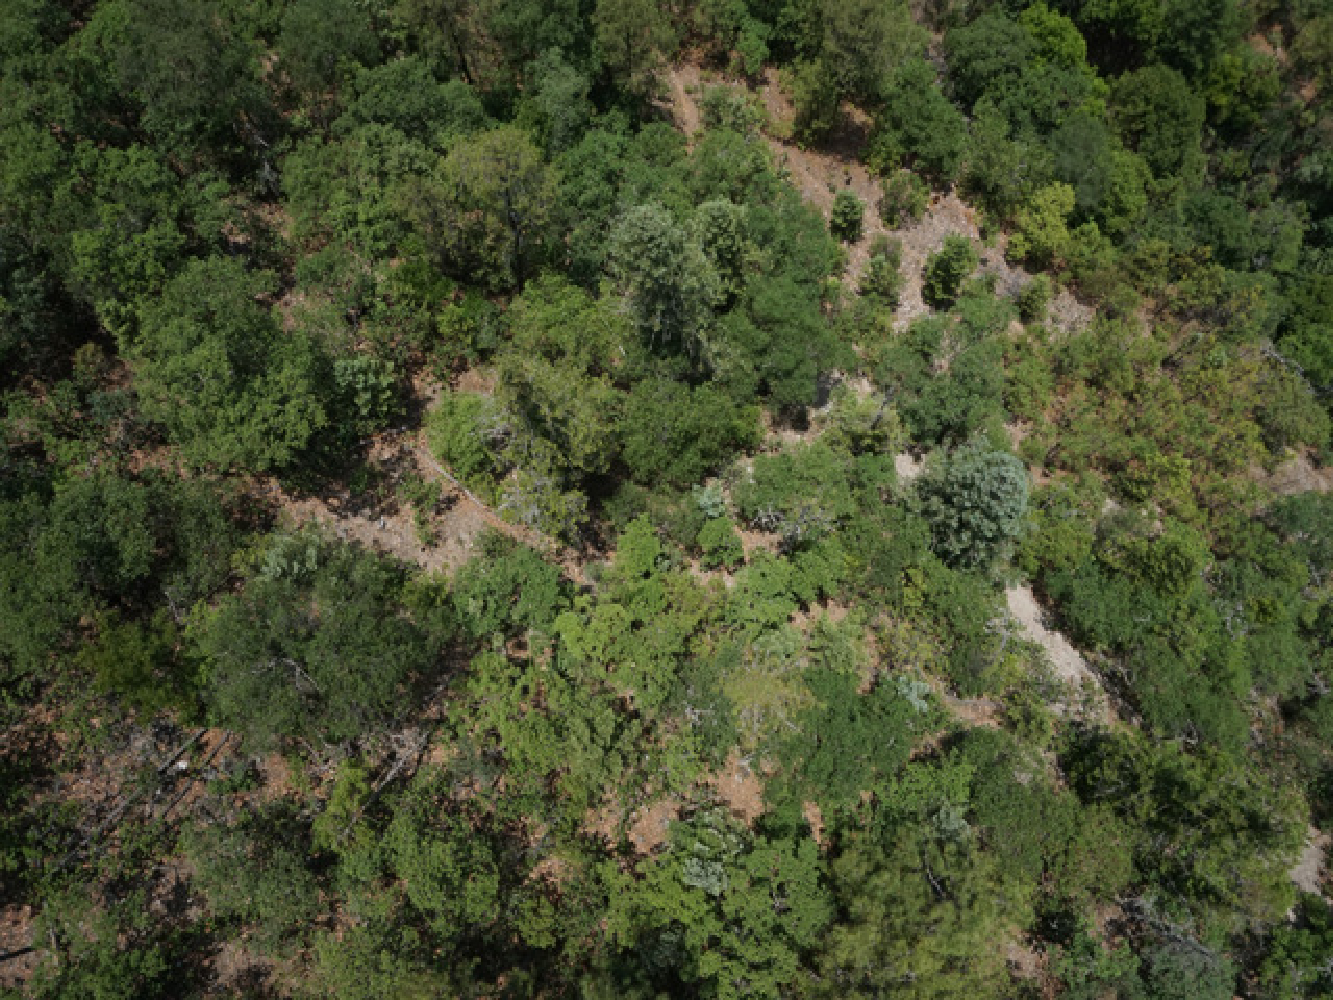
\includegraphics[width=0.45\textwidth]{DSC06100}} & 
\subfloat[Histograma generado]{\includegraphics[width=0.45\textwidth]{histograma-gen}} &
  \end{tabular}
  \caption[Histograma de color]{Histograma de color generado con las bibliotecas \texttt{matplotlib y OpenCV.}}
  \label{Histograma-generado}
\end{figure}


\subsection{Forma}
La característica de forma cuenta también con varias métricas, se hace énfasis en los \emph{momentos de una imagen}. 
Los momentos de una imagen son los pesos promedio de la intensidad de píxel sobre una imagen.  

\begin{figure}[h!]
  \centering
  \begin{minipage}[b]{0.8\textwidth}
    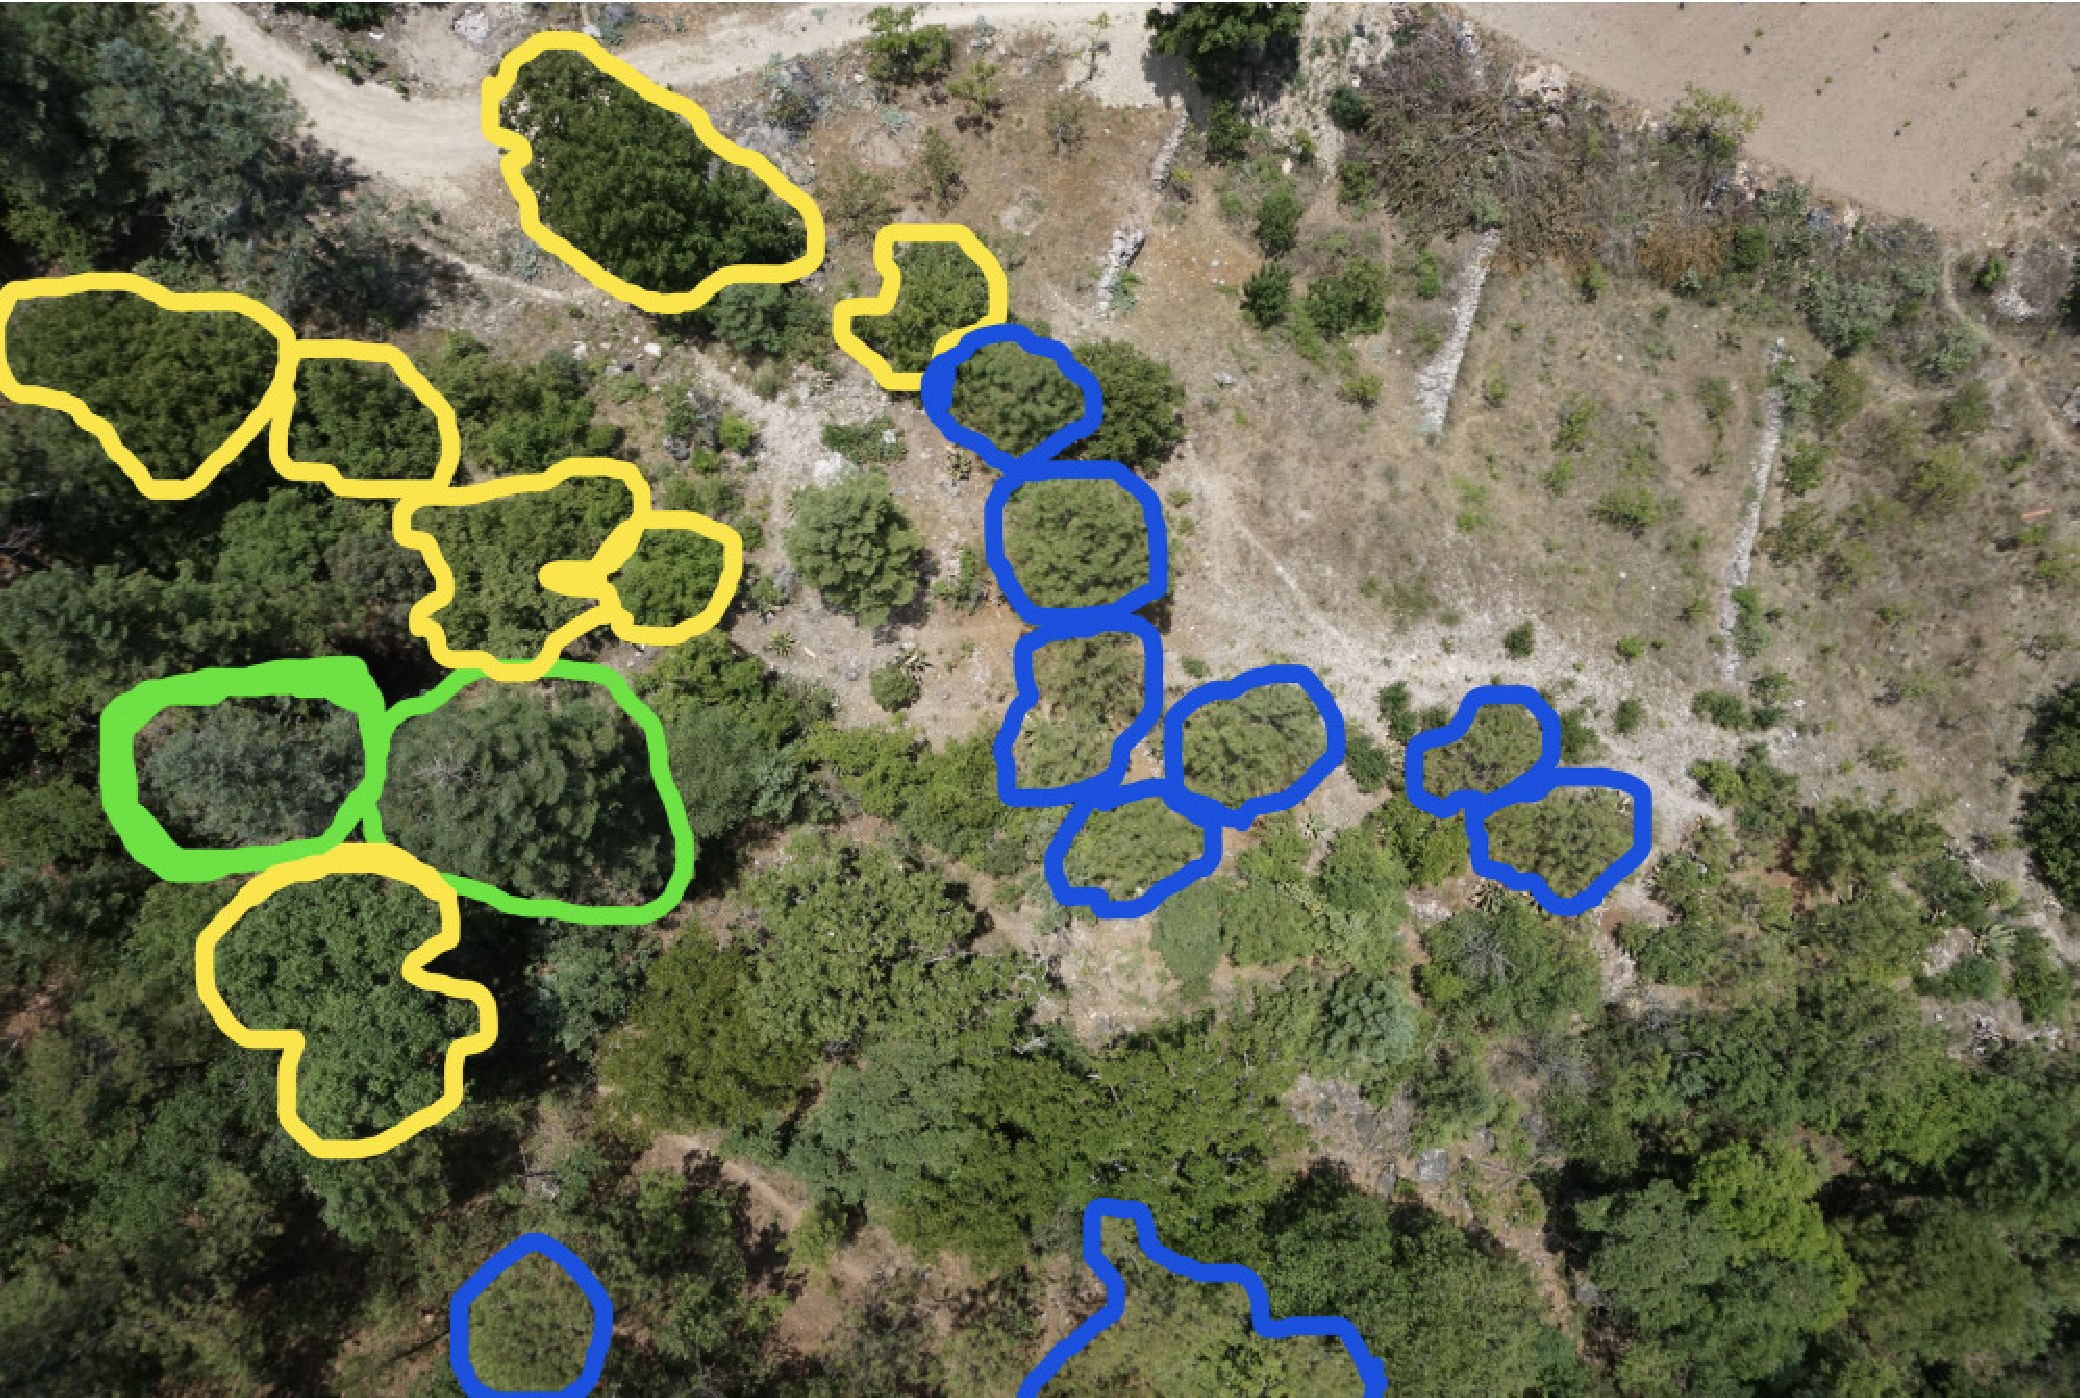
\includegraphics[width=\textwidth]{Anotaciones-ex}
    \caption[Formas de cada especie arbórea.]{Formas de cada especie arbórea (verde: Abies, azúl: Pino, amarillo: Encino).}
  \end{minipage}
\end{figure}

Por ejemplo, el canal $I$ de una imagen contiene una intensidad en los ejes $(x,y)$ dados por la ecuación $I(x,y)$ donde $I(x,y)$ hace referencia una imagen binaria donde sólo es posible tomar un valor cero o uno. En otras palabras, los momentos de una imagen son un conjunto de siete números calculados del movimiento central que son invariantes para las transformaciones de una imagen
\begin{equation}
\label{eq:2.1}
 M = \sum_{x}\sum_{y} I(x,y).
\end{equation}

La ecuación \ref{eq:2.1} obtiene la sumatoria de la intensidad de todos los píxeles, es decir, la sumatoria se hace con base únicamente en la intensidad de los píxeles y no con la posición dentro de una imagen.

\subsection{Textura} 
Esta característica tiene una gran relevancia dado que es de las más usadas al momento de identificar objetos en regiones de interés en fotografías aéreas, micrográficas y de satélite y en el presente trabajo, al identificar las muestras de los árboles. En este caso se emplea la métrica de \emph{textura de Haralick}. 

La figura 2.3 ilustra las distintas texturas que tienen los especies arbóreas en la imagen, a simple vista algunos colores denotan ser de una especie distinta si se hace un análisis minucioso, pero en este caso, la característica de textura puede ser utilizada para diferenciar entre especies arbóreas.
\vspace*{3\baselineskip}
\begin{figure}[h!]
  \centering
\begin{tabular}{@{}ccc@{}}
\subfloat[Encino]{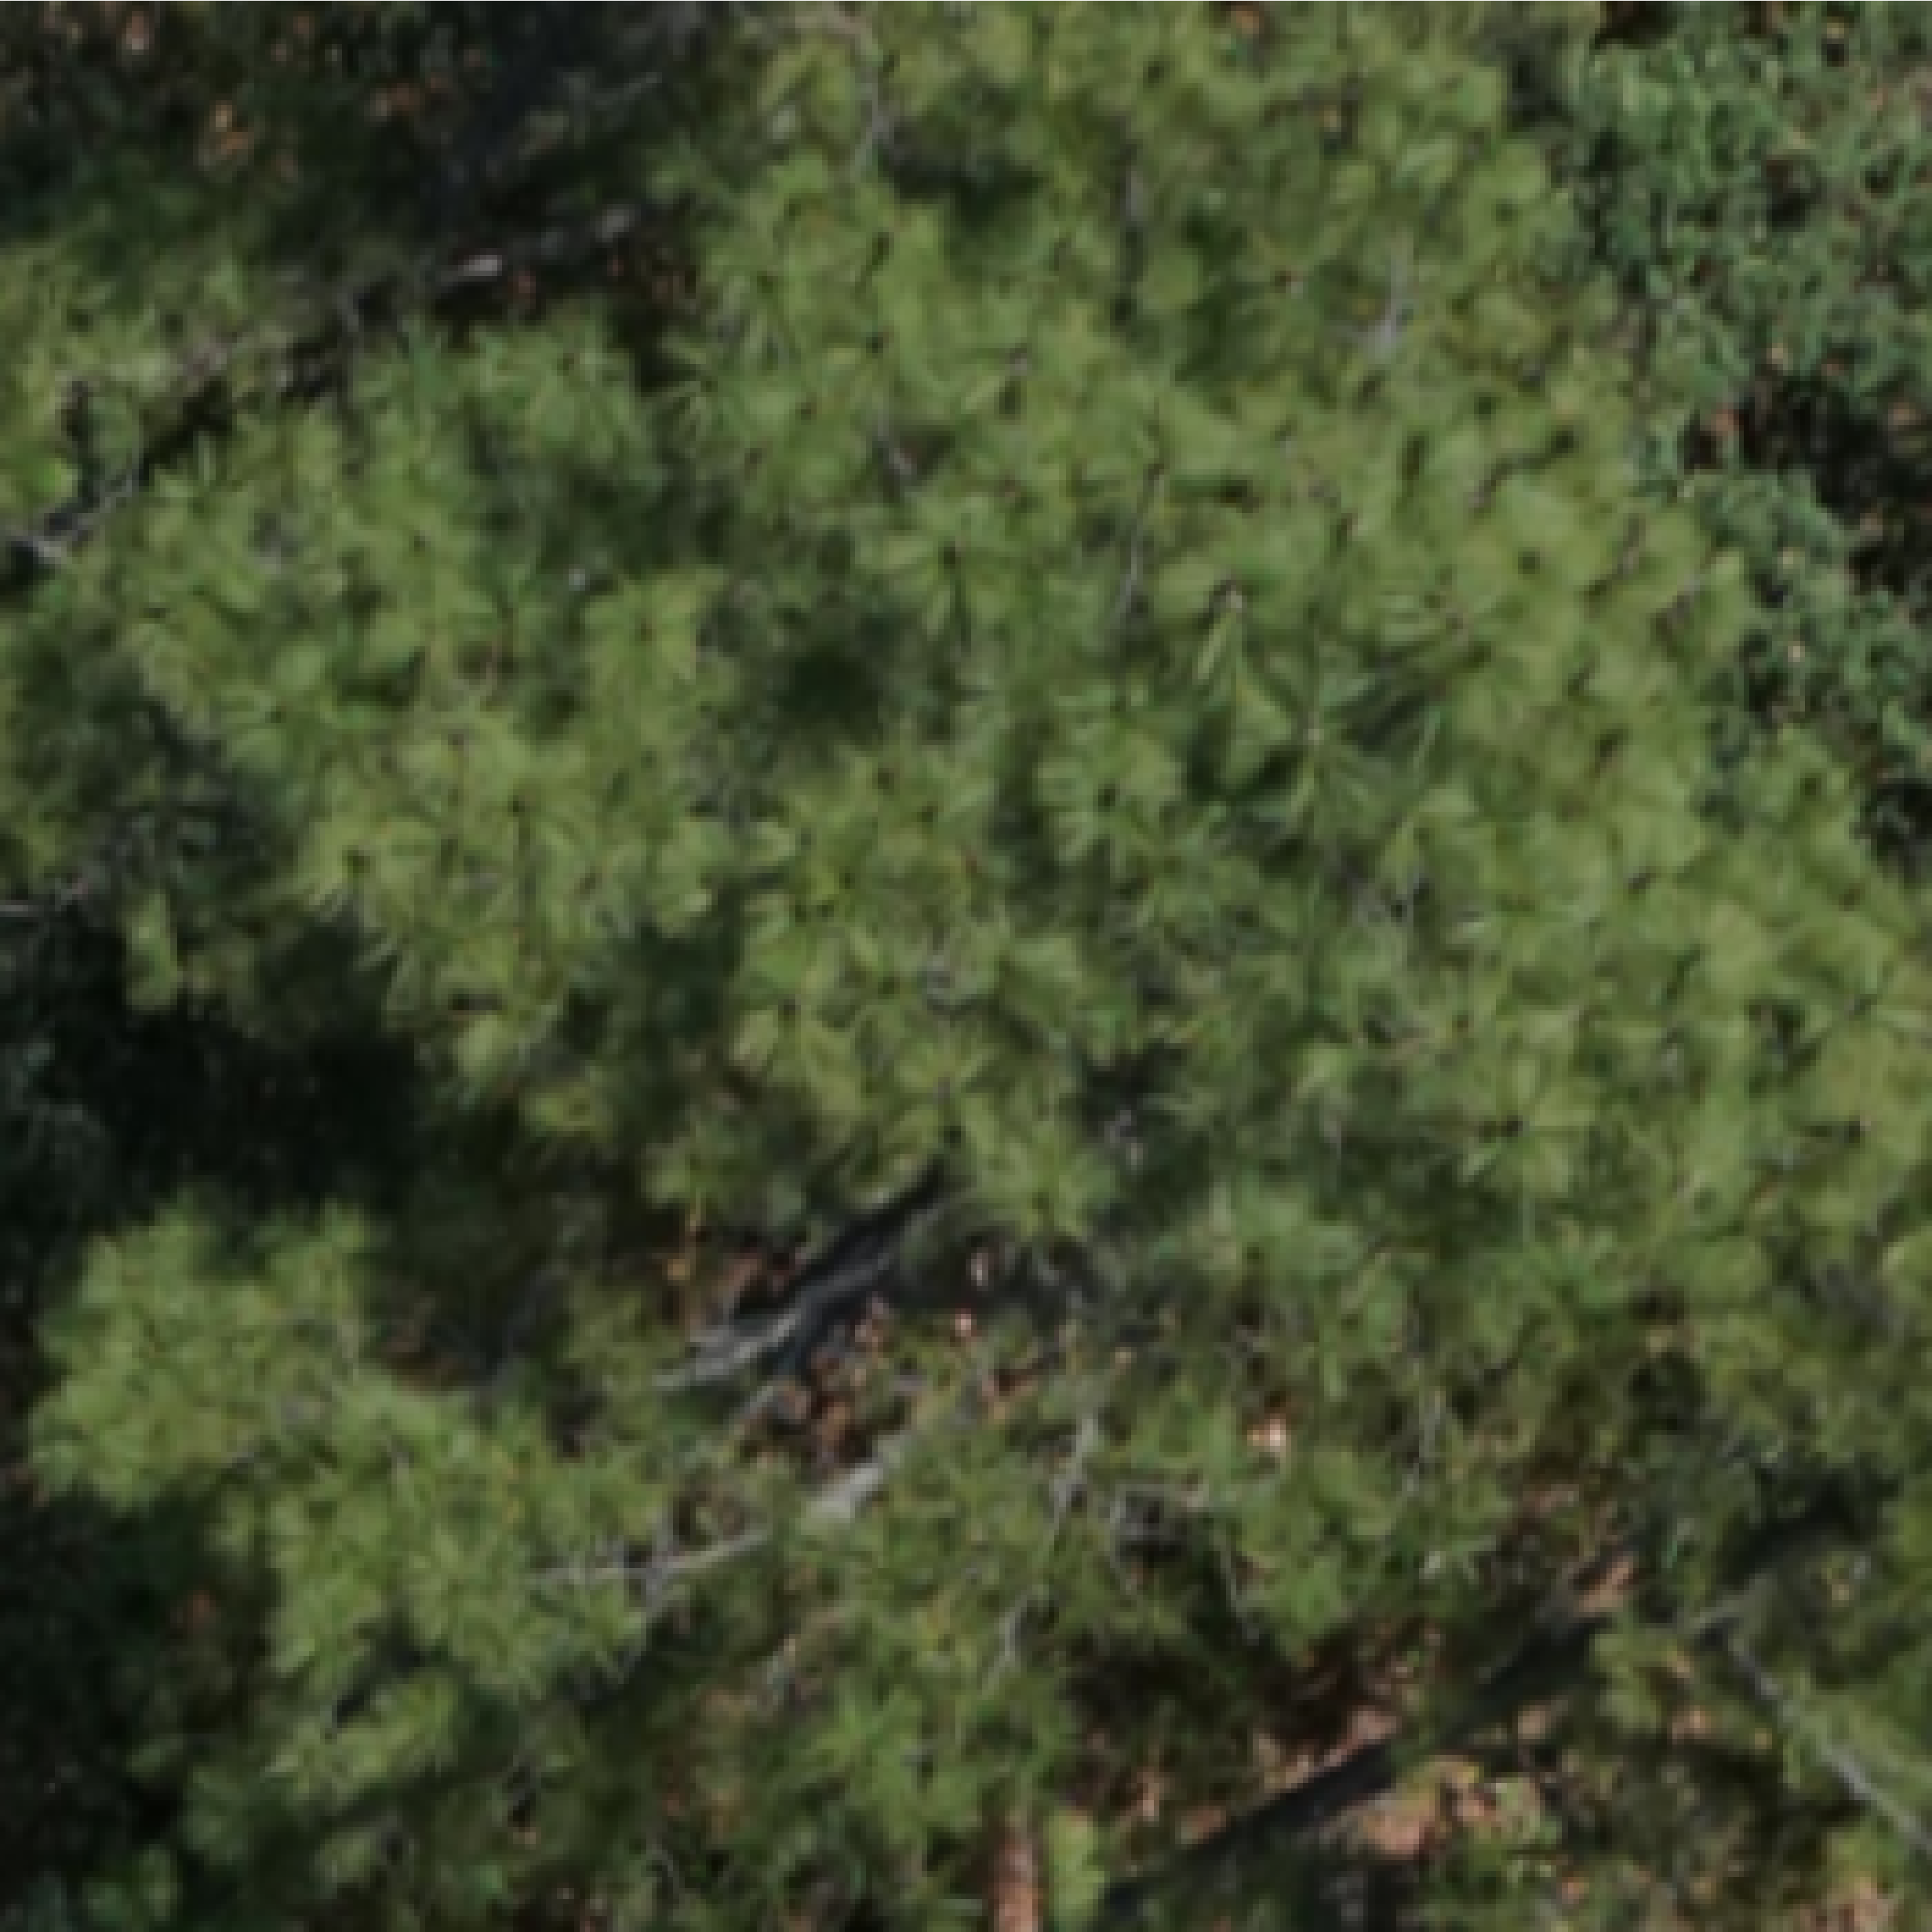
\includegraphics[width=0.3\textwidth]{1_res}} & 
\subfloat[Pino]{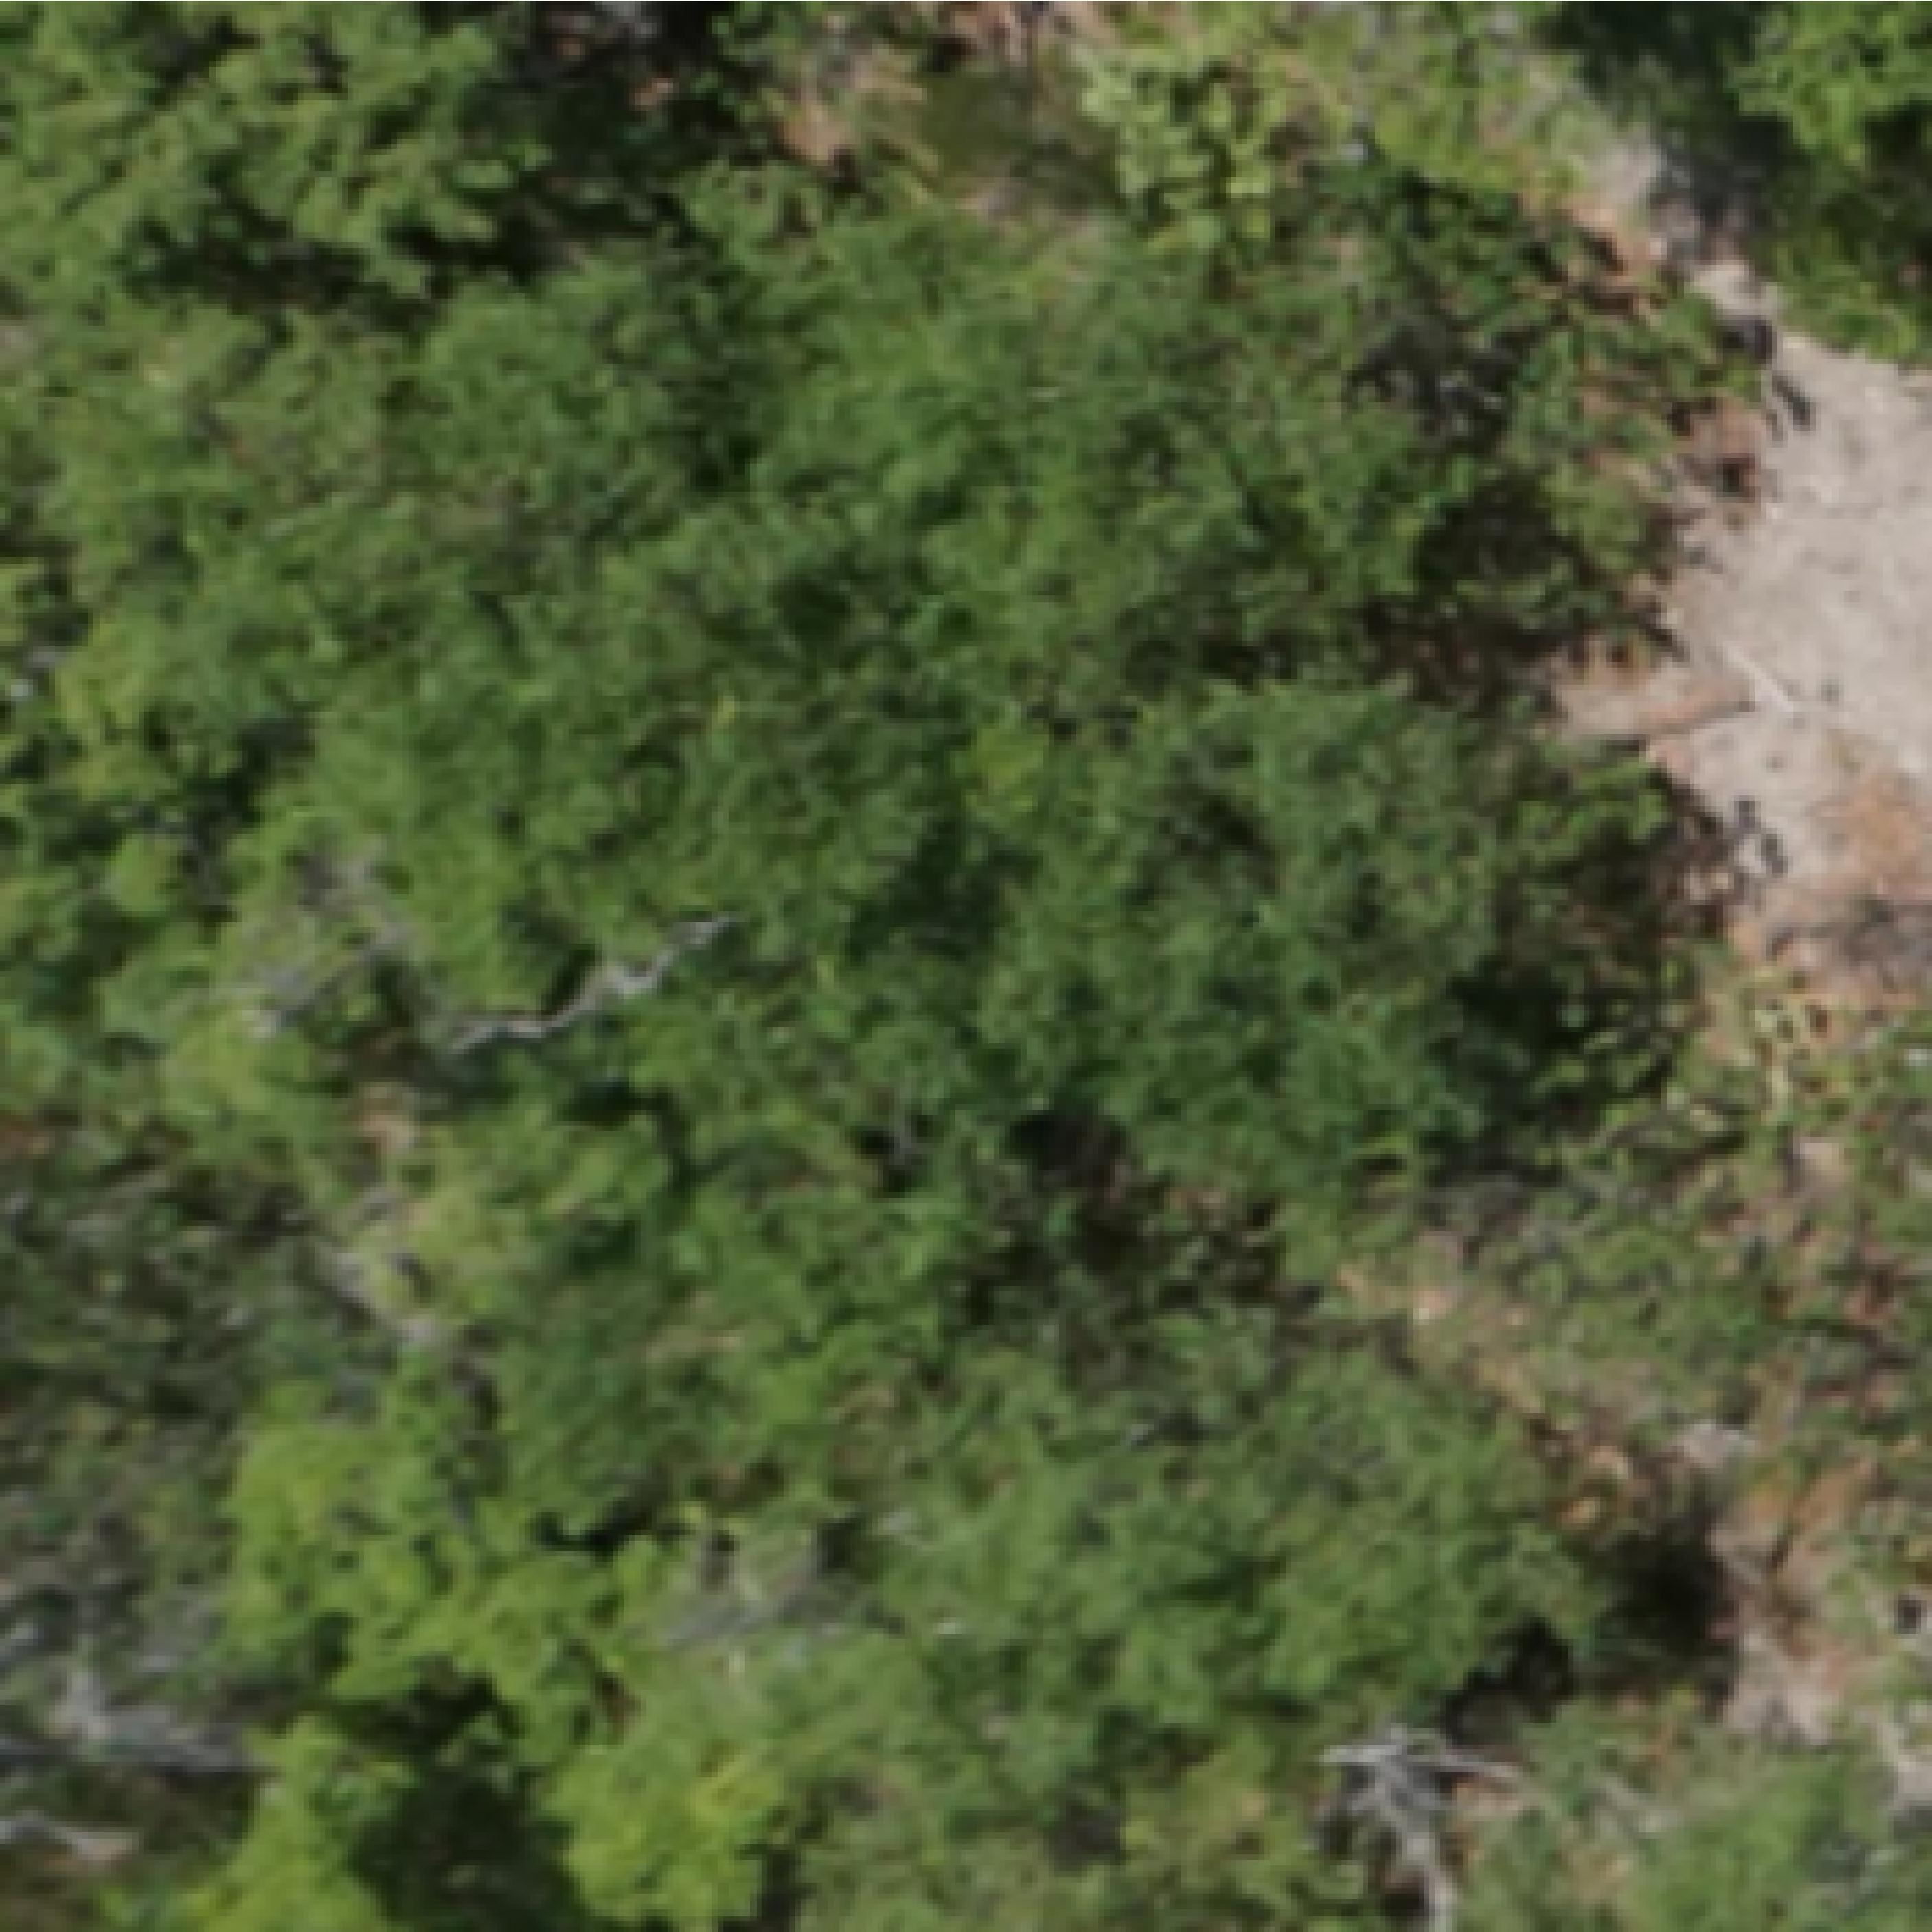
\includegraphics[width=0.3\textwidth]{2_res}} &
\subfloat[Abies]{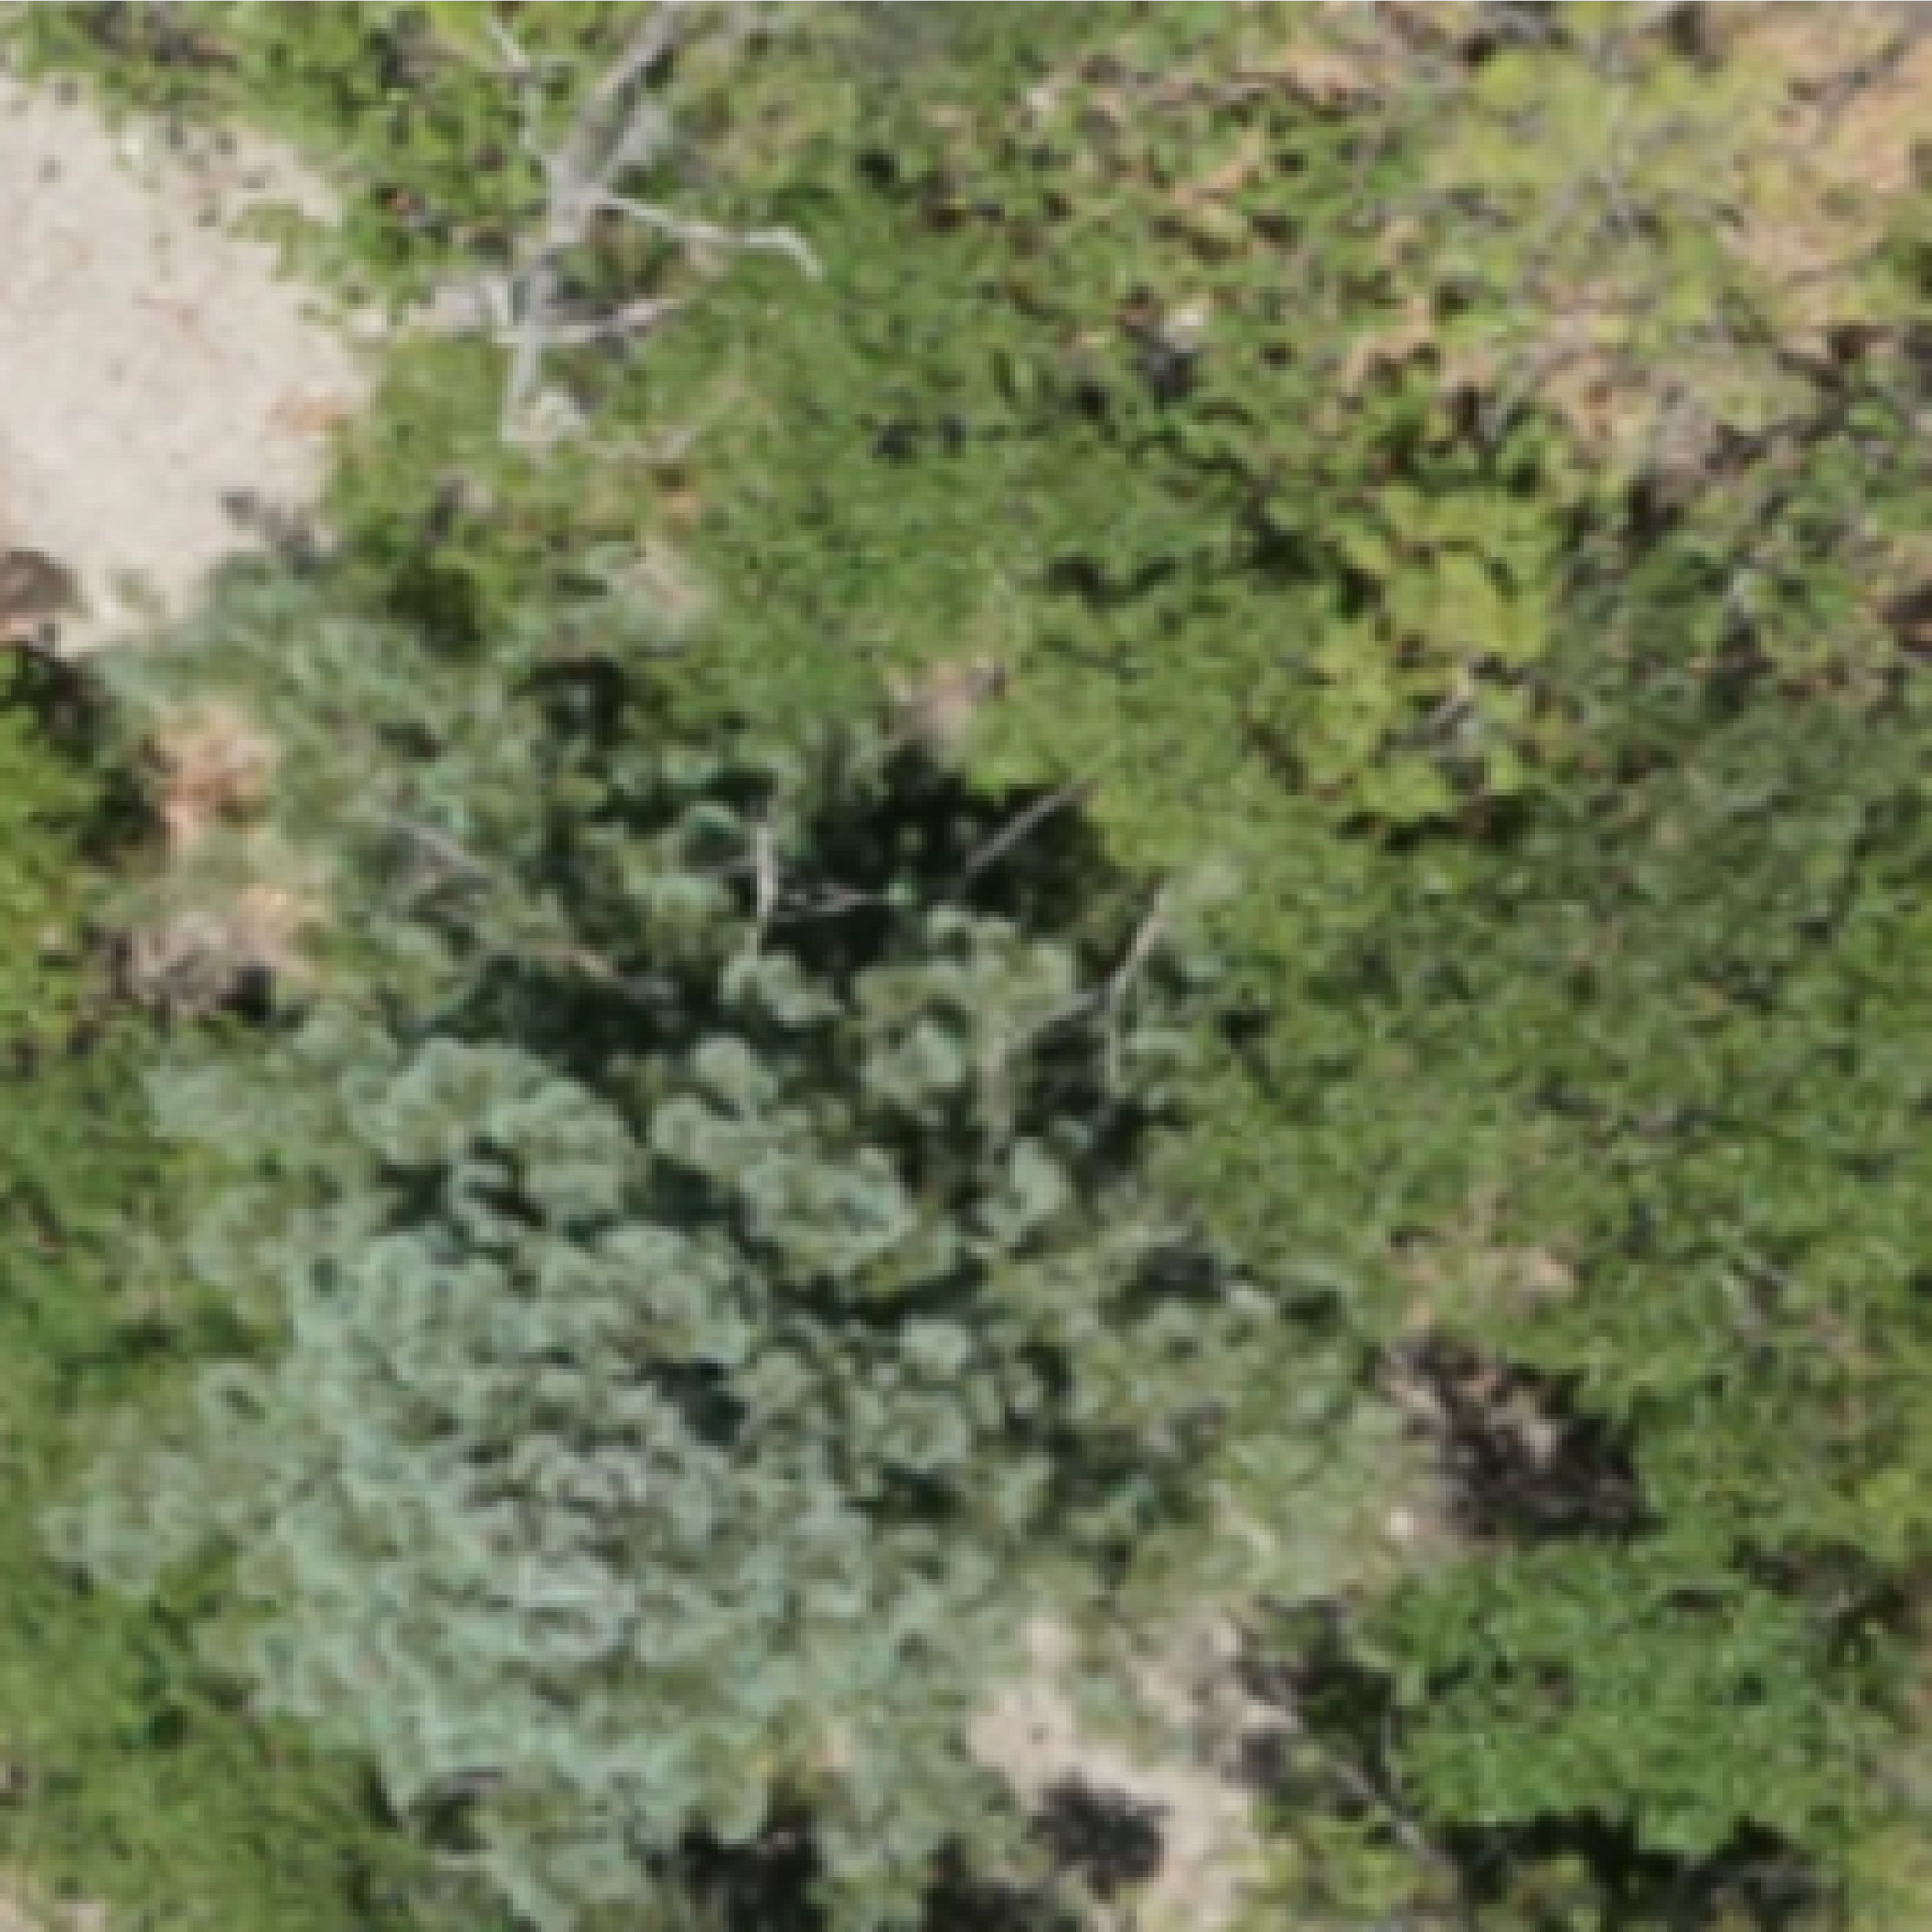
\includegraphics[width=0.3\textwidth]{3_res}}
  \end{tabular}
  \caption[Comparación de texturas.]{Comparación de texturas encontradas.}
  \label{Texturas}
\end{figure}
\newpage
\section{Descriptores de características locales}
Las características mencionadas en la sección 2.2 cuantifican globalmente una imagen, sin embargo, para poder determinar las características que cuantifican localmente las regiones de una imagen es necesario determinar que descriptor es el óptimo para describir los puntos de interés de una imagen completa o los puntos de interés de cierta región de la imagen. 

\begin{description}
\item[SIFT (Característica de transformación de escala invariante)]{Extra la información de una imagen para posteriormente, permita adecuarla cuando se desee compararla con diferentes muestras de un objeto o escena.}
\end{description}

\begin{description}
\item[SURF (Característica de acelerado robusto)]{Toma un vecino al rededor del punto seleccionado en la imagen y es dividido en sub-regiones para cada sub-región, la respuesta de la transformada de Wavelet es tomada y representada por esta característica.}
\end{description}
 
\begin{description}
\item[BRIEF (Características elementales  independientemente binarias robustas)]{Se enfoca en la orientación de una imagen y depende del menor numero de diferencias (puntos) a su alrededor.}
\end{description}

\begin{description}
\item[ORB (BRIEF Rotada y orientada rápida)]{Se relaciona con BRIEF debido a
que esta es una fusión de la ya mencionada con un punto detector clave rápido (FAST). Para determinar estos puntos clave rápido, se utiliza FAST y posteriormente, la medida de esquinado de Harris es aplicada para encontrar los $n$ puntos más altos. En concreto, esta característica registra la intensidad ponderada del centroide la cual está localizada en la esquina de un centro.}
\end{description}

\section{Uso de los descriptores}
Existen varias formas de utilizar los descriptores pero hay dos maneras de mezclar las características de vectores.

\paragraph{•} Para las características globales de vector, sólo se concatena cada característica del vector para formar a una característica global del vector simple. Este enfoque se utiliza en el desarrollo de este algoritmo.

\paragraph{•} Para las características locales del vector también puede hacerse una combinación de las características locales y globales del vector, es necesario algo llamado \emph{modelo de la bolsa de palabras} (BOVW). Este enfoque se utiliza normalmente en constructores de vocabularios, agrupamiento de $K$-medias, etc.

\paragraph{•} El \emph{escalamiento} es también otra de los descriptores utilizados en las características de los vectores, este sirve para transformar los datos de las características en rangos específicos de cero a uno, por ejemplo. Esta característica suele ser bastante usada en máquina de soporte vectorial y en el $K$-vecinos cercanos (KNN) donde la distancia entre dos puntos es importante.

\paragraph{•} La \emph{normalización} es utilizada en los descriptores también, esta última es una técnica donde los valores son desplazados y re-escalados  para que puedan alcanzar un rango entre cero y uno, a esta característica también se le conoce como \emph{escalamiento mínimo-máximo}.

\chapter{Estado del arte}
En este capítulo se explica la relación de la investigación en curso con investigaciones de otros autores, la importancia de la visión computacional y su relación con los inventarios forestales, así como los apartados que se desarrollan durante la investigación.

\section{Investigaciones relacionadas}
Existen algunos trabajos que no están completamente relacionados con el objetivo de identificar especies arbóreas, pero si existen investigaciones que toman como objetivo el analizar zonas forestales.

Este artículo menciona como hacen uso de combinar datos para realizar inventarios forestales por medio de sistemas digitales aéreos de fotogrametría y escáneres láser. Con estas tecnologías, hacen una búsqueda buscando los tipos predominantes en una zona y con ayuda del \emph{análisis de imágenes basado en objetos} se pudo admitir la delineación automática de árboles, la clasificación de especies arbóreas y la definición de atributos estructurales a nivel de árbol. 
\newline
\break


\citet{rf1} utilizan una gran cantidad de entradas para definir manualmente la especie, no obstante, la principal diferencia es que este trabajo no realiza por medio de visión computacional sino por técnicas tradicionales.
 
\citet{rf2} tienen como meta evaluar artículos para actualizar los inventarios de árboles en un área metropolitana. En este no se trata con inteligencia artificial como tal, pero si hacen uso de tecnologías de detección como sensores remotos que permitan evaluar correctamente y obtengan la información concreta de las zonas donde habitan  árboles.

\citet{rf3} tienen como objetivo detectar objetos además de hacer uso del umbral adaptativo, el cual es muy utilizado en la visión computacional. %El problema a solucionar en concreto como parte de este trabajo es, resolver los métodos de umbralización.

\citet{rf9} hace simulaciones para la gestión de modelos forestales que podría ser requeridos para la toma de decisiones en un sector forestal. En este artículo se hacen validaciones usando modelos generados por información de un bosque privado y un bosque estatal de Illinois, EE.UU.

\citet{rf10} hacen uso de técnicas de inteligencia artificial para la identificación  de especies forestales haciendo uso de multidatos espectrales tomando como punto de partida, los vecinos más cercanos (KNN) para procesar eficientemente la información recolectada y segmentar por clusters el ambiente sobre el que se trabajó.

\pagebreak
 
\section{Comparación de trabajos}
La mayoría de los trabajos citados hacen uso de otra clase de tecnología que no tiene que ver directamente con la utilizada en nuestra investigación, más sin embargo, algunos de los aspectos clave que se presentan en nuestra investigación con respecto a las investigaciones encontradas son:

\begin{description}
\item[Inventarios forestales]{ Son aquellos que permiten tener un control de las especies que pueblan una zona específica.}
\end{description}

\begin{description}
\item[Análisis de imágenes]{Es una técnica bastante utilizada hoy en día por la visión computacional para extraer datos e información de imágenes.}
\end{description}

\begin{description}
\item[Visión computacional]{Este concepto está completamente relacionado con la inteligencia artificial, dado que es una  técnica del aprendizaje máquina que busca encontrar objetos emulando la capacidad humana del reconocimiento.}
\end{description}

\begin{description}
\item[Clasificación]{Es el acto de separar u ordenar bajo un criterio específico.}
\end{description}

\begin{description}
\item[Especies]{Son los distintas categorías o  clases de algún objeto en particular.}
\end{description}

\begin{description}
\item[Zonas]{Es algún sector o delimitación de territorio de algún sitio, ciudad, país.}
\end{description}

\begin{description}
\item[Detección de objetos]{Es una técnica del aprendizaje máquina que emula la capacidad humana de detectar por si sola, algún objeto por medio de la vista.}
\end{description}

\newpage

\subsection{Comparaciones}
En el cuadro \ref{tab:Comparación de trabajos frente al desarrollado}, se desglosan que características presentes  que se pueden encontrar en las investigaciones citadas y su relación con la investigación con la que se está trabajando actualmente.\\
\renewcommand{\tablename}{Cuadro}
\begin{table}[hbt!]
	{\centering
	\caption{Comparación de trabajos frente al desarrollado. \checkmark: cumple con esta característica, $\times$: no cumple con esta característica.}
	\begin{adjustbox}{width=\textwidth}
		\begin{tabular}{|c|c|c|c|c|}
			\hline
			 Trabajos &  Inventarios forestales &  Visión computacional & Detección de objetos\\
			\hline
			\citet{rf1} & \checkmark & $\times$ & \checkmark \\
			\hline
			\citet{rf2}&  \checkmark  &  $\times$ & $\times$  \\
			\hline
			\citet{rf3}& $\times$ & \checkmark & \checkmark  \\
			\hline	
			\citet{rf9}& \checkmark & \checkmark & \checkmark  \\
			\hline
			\citet{rf10}& $\times$ & \checkmark & \checkmark  \\
			\hline
			\citet{rf11}& $\times$ & \checkmark & \checkmark  \\
			\hline
			\citet{rf12}& \checkmark  & $\times$ & $\times$  \\
			\hline
			\citet{rf13}& \checkmark & $\times$ & $\times$  \\
			\hline
			\citet{rf14}&  $\times$ & \checkmark & $\times$   \\
			\hline
			\citet{rf15}& \checkmark & \checkmark & $\times$  \\
			\hline
			El presente trabajo & \checkmark & \checkmark & \checkmark \\
			\hline
		\end{tabular}
	\end{adjustbox}
	\label{tab:Comparación de trabajos frente al desarrollado}}
\end{table}

\subsection{Áreas de oportunidad}
En el cuadro 3.1 se puede apreciar que características tiene la investigación con respecto a la de otros autores, y es que pudiera ser que otros trabajos tengan las mismas características o al menos casi todas pero por lo que respecta a la investigación, además de generar un inventario forestal de manera eficiente y proporcionar su código, este puede ser modificado o estudiado con otros propósitos sin necesidad de esperar una retribución de por medio debido a que es un software libre.

Por otro lado, también se puede apreciar que el trabajo de \citet{rf10} tiene las mismas características que el método propuesto, sin embargo va orientado a otro objetivo, que es tomar decisiones. Sin embargo, las herramientas descritas en el artículo no son de uso gratuito, permitiendo así, otorgar la ventaja de que la investigación sea de licencia abierta respecto a esta investigación.

En lo que respecta a las áreas de oportunidad de la investigación, se puede destacar el aprendizaje máquina y la visión computacional como herramientas clave. Primeramente, el aprendizaje máquina permite entrenar un algoritmo cuyo producto es bastante relevante en el proceso de clasificación durante la investigación.

En el caso del método propuesto, el aprendizaje máquina se encarga de extraer información clave de cada una de las muestras recolectadas de las zonas forestales, donde, mediante descriptores de características tanto globales como locales, se encarga de generar un archivo que contenga la información más relevante de las muestras.

Posteriormente, la visión computacional hace uso del archivo generado previamente por el aprendizaje máquina donde se encarga de clasificar cada árbol mediante una etiqueta que define a su especie por color. Esto último no ha sido aplicado en las investigaciones encontradas puesto que tienen un enfoque nulo en hacer clasificaciones de múltiples objetos de un sólo tipo, o bien, sólo se enfocan en hacer anotaciones manuales por medio de inputs previamente establecidos y esto únicamente se enfoca en comparaciones.

El inventario forestal es otro de los apartados importante en la investigación, dado que es uno de los enfoques en los que se el desarrollo de los algoritmos que se utilizan, se está tomando como punto de partida al momento de desarrollarse. 

Clasificación es quizás el punto más importante de la investigación debido a que, se hace un análisis de las muestras recolectadas previamente por los drones y posteriormente, haciendo uso de la visión computacional y el aprendizaje máquina se entrena el modelo que hace la clasificación de especies arbóreas.


\chapter{Solución propuesta}
Habiendo conocido las características que mejor describen a los atributos del presente trabajo, se puede decir que la base del método propuesto se puede desarrollar.

\section{Fase de recolección de muestras}
La primera fase en el desarrollo de la solución propuesta sería recolectar muestras de el objeto(s) a identificar por medio del aprendizaje máquina. Si bien es necesario tener una gran cantidad de muestras para que el presente trabajo tenga una perspectiva más amplia de lo que se necesita reconocer, también hay que considerar que se necesita información que contenga la menor cantidad de información no útil dado que esto podría sobre entrenar al modelo que se encargue de la clasificación.

\newpage
\section{Muestras recolectadas}
Inicialmente, el doctor Manuel Jiménez proporcionó un repositorio con imágenes alojado en Google Drive que contenía imágenes de las zonas donde se realizó el recorrido del dron, más específicamente \emph{Cilantrillo} y \emph{Trinidad}.

\begin{figure}[h!]
 \centering
 \subfloat[Ejemplo de muestras de la zona de Cilantrillo]{\includegraphics[scale=0.150]{grid_Cilantrillo}}\par
\subfloat[Ejemplo de muestras de la zona de Trinidad]{\includegraphics[scale=0.150]{grid_Trinidad}}
\end{figure}

\newpage
\subsection{Análisis de muestras}
Como se mencionó al inicio de la sección 4.2, es importante recolectar una gran cantidad de muestras para entrenar bien el modelo, por lo que para la zona del Cilantrillo se recolectaron 277 muestras y para la zona de Trinidad se recolectaron 270 muestras. Esta cantidad de muestras es suficiente para entrenar bien el modelo desarrollado y que sea capaz de reconocer los distintos tipos de árbol, más sin embargo, en cada imagen se puede apreciar información que no es útil y puede sobre entrenar el modelo, perjudicando de forma que este detecte más en concreto, el suelo como un tipo de árbol.

La información de cada muestra es analizada píxel por píxel, por lo que a simple vista se puede percibir la clase de información que contiene cada muestra, pero el analizar cada una de ellas llevaría demasiado tiempo, por lo que, se puede concluir que hay píxeles dentro de ellas que no sean útiles. 

En los casos de la figura 4.3 y 4.4 se muestra un ejemplo de cómo se verían las muestras que son de utilidad y destacando que en el siguiente capítulo define el procedimiento realizado para poder obtener muestras útiles.


\begin{figure}[h!]
  \centering
\begin{tabular}{@{}ccc@{}}
\subfloat[Muestra no útil]{\includegraphics[width=0.48\textwidth]{DSC06080}} & 
\subfloat[Muestra útil]{\includegraphics[width=0.48\textwidth]{DSC06080-sf-2}} &
  \end{tabular}
  \caption[Comparación de muestras]{Comparación de muestras donde se aprecia una útil de una no útil.}
  \label{Comparación de muestras}
\end{figure}
\newpage

\subsection{Información no útil}
En cada una de las muestras recolectadas está presente el suelo ya que es una imagen capturada por un drone, sin embargo, el suelo forma parte de la información que se necesita remover de las muestras para no sobre entrenar a el modelo de reconocimiento previamente desarrollado.

Para efectos prácticos, se declaran los colores de las especies arbóreas, esto con el fin de decirle a el método propuesto que información no debe remover de las muestras. A su vez se tiene que declarar que la información se reemplaza con píxeles transparentes. Cabe destacar que nuestras imágenes no cuentan con un canal de transparencia, mismo que es necesario para llevar a cabo el método propuesto de reemplazar la información, por lo que se tiene que convertir cada muestra primero, a un formato \texttt{.png} para que la muestra admita este canal. Después se convierte la muestra a un canal \emph{RGBA} (Red Gray Blue Alpha).

 Una vez que la muestra tenga el canal transparente, se recorren todos los píxeles de la imagen con el fin de encontrar y asignar a una variable, todos los pixeles que no correspondan con los colores de los árboles y posteriormente, descartar estos píxeles con el fin de guardar la muestra con la información útil como se muestra en la figura 2.5.

\begin{figure} [!h]
	\centering
	\begin{minipage}[b]{0.65\textwidth}
		\includegraphics[width=\textwidth]{DSC06080-sf-2}
		\caption{Resultado de remover píxeles}
	\end{minipage}
\end{figure}

\break

\section{Fase de procesamiento de muestras}
Una vez recolectadas las muestras con información relevante, se procede a  entrenar a el modelo con esa información para que sea en fases posteriores este sea capaz de entender y clasificar donde estén presentes las especies arbóreas almacenadas en el modelo. La forma de organizar cada muestra para un correcto entrenamiento es mediante la separación de cada especie por su color correspondiente, es decir, separando las especies de color azul en una carpeta, los verdes y los amarillos en su carpeta correspondiente consecuentemente.

\subsection{Recortando muestras por islas}
Primeramente hay reconocer las secciones o partes de la muestra que son de interés, en este caso, se trabaja con los colores, específicamente los de cada especie de árbol. En el caso de todas las muestras, se tienen tres colores: [verde, amarillo, azul]. Estos colores indican que colores tienen una anotación válida para recortar.


\begin{figure}[H]
  \centering
  \begin{minipage}[b]{0.65\textwidth}
        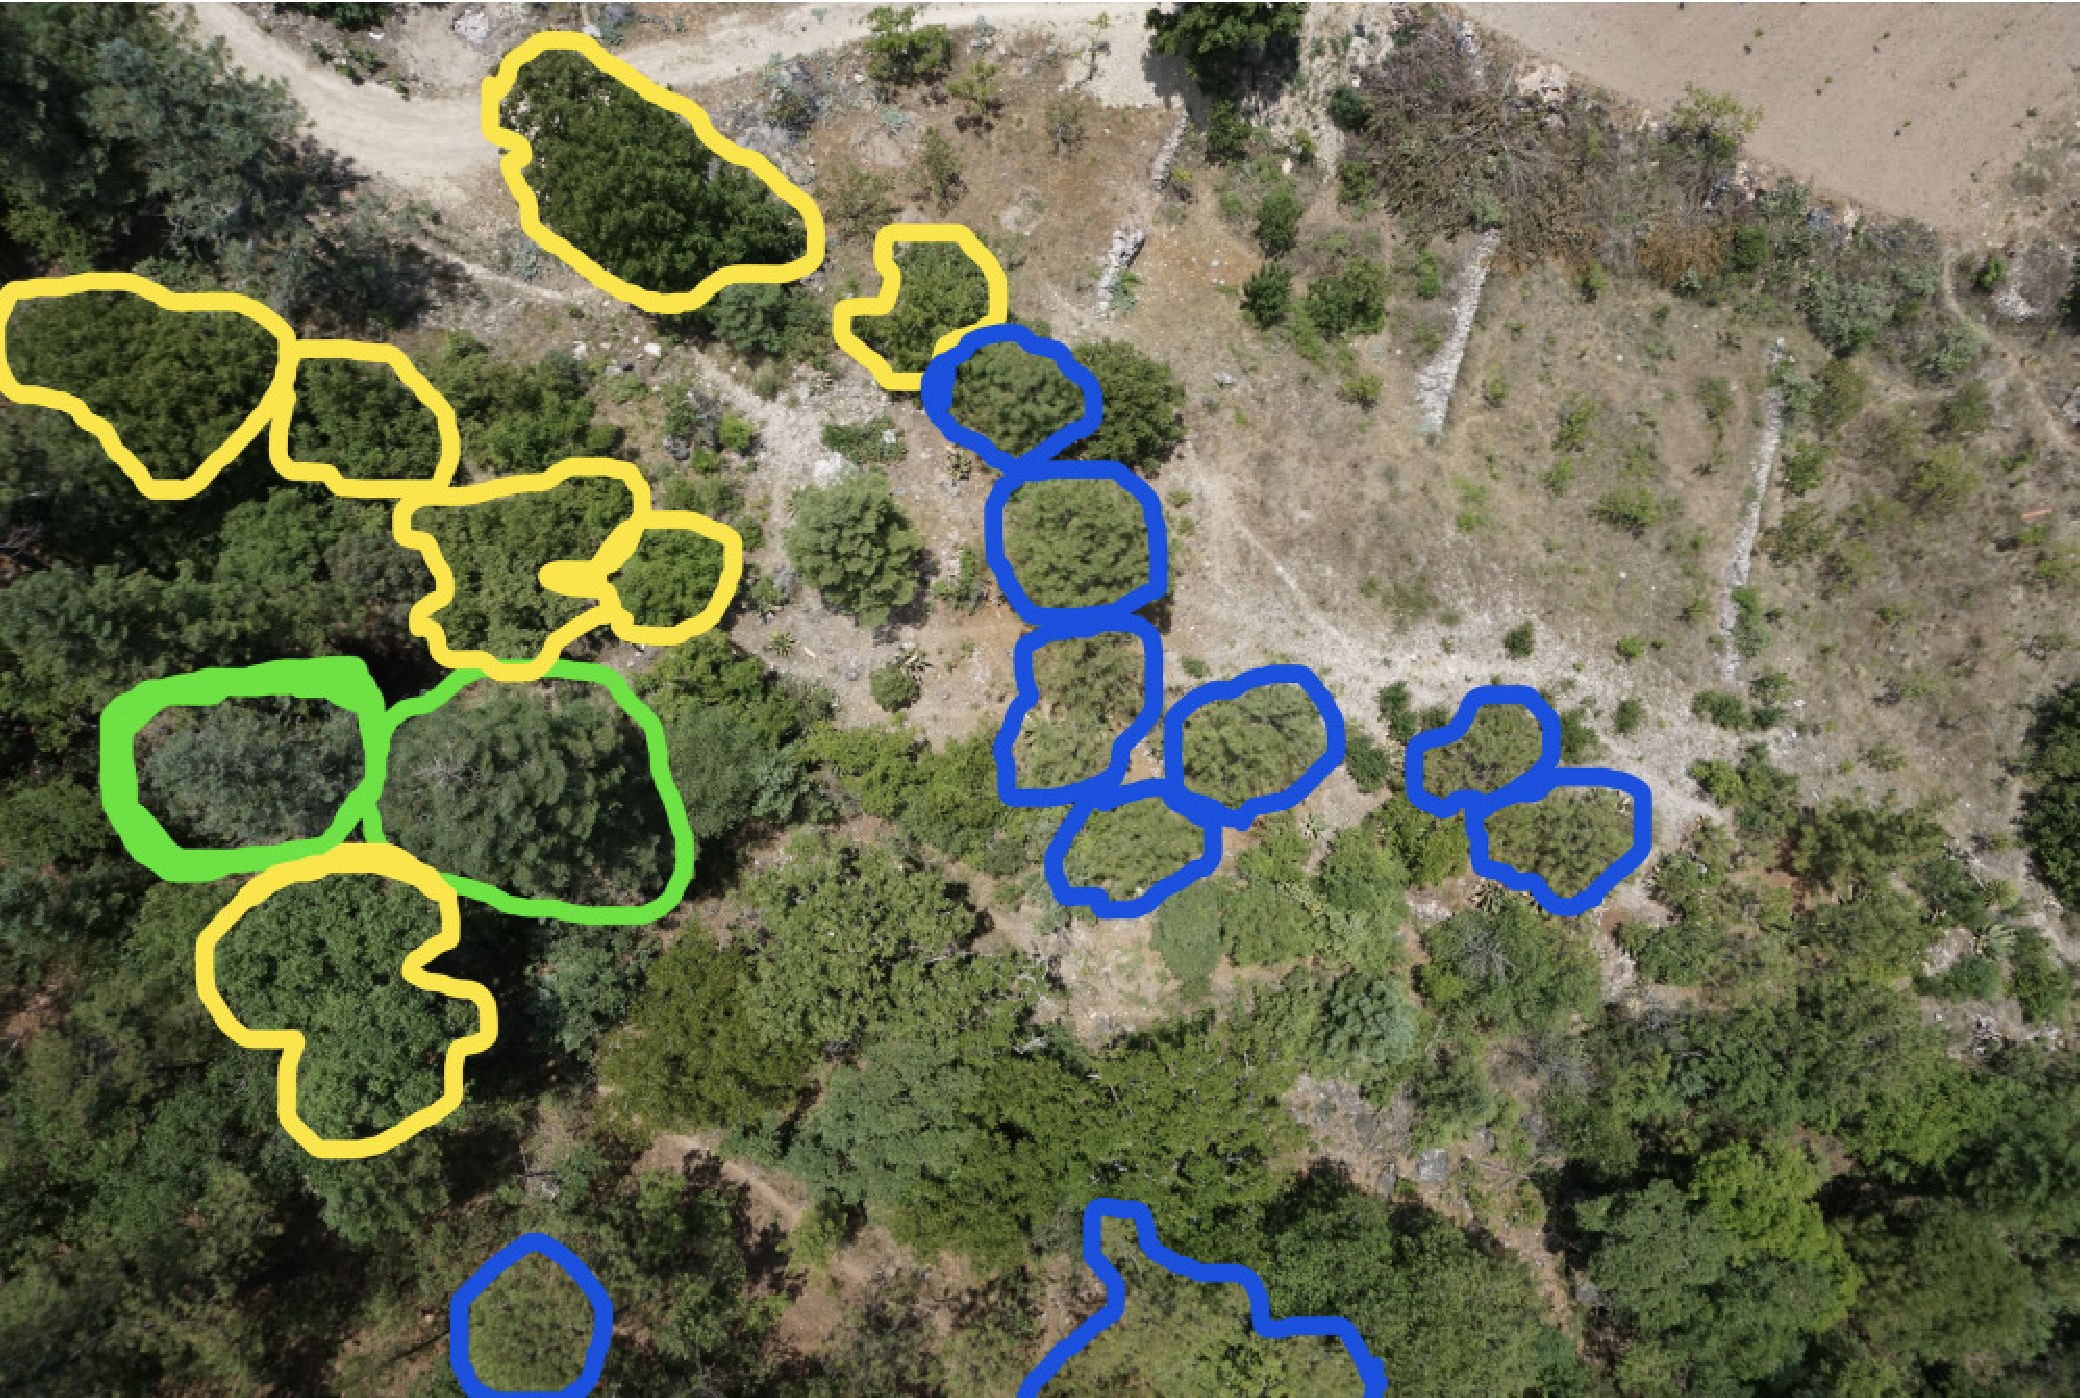
\includegraphics[width=\textwidth]{Anotaciones-ex}
    \caption{Muestra con anotaciones}
  \end{minipage}
\end{figure}
\newpage

En la figura 4.6 se aprecia que tiene secciones delimitadas por colores, por lo que se recorre la muestra por píxeles hasta encontrar la zona que esté dentro del rango de colores previamente establecido.

La idea de hacer recortes de las anotaciones por colores es de agilizar el procesamiento a la hora de entrenar el modelo con todas las muestras. Cada muestra a su vez, tiene un porcentaje de admisión que permite establecer si la anotación cumple o no con los criterios establecidos.

Ya con las muestras de colores obtenidas, se procede a separar por islas de acuerdo al color que este establecido. Se separa por color verde, amarillo y azul, cada color en una carpeta distinta para tener mayor control de las islas capturadas.

\begin{figure}[H]
  \centering
  \begin{minipage}[b]{0.6\textwidth}
        \includegraphics[width=\textwidth]{grid_Muestras_2}
    \caption{Isla separada por color}
  \end{minipage}
\end{figure}

En la figura 4.7 se aprecian las islas separadas por color, en cada una de estas muestras, se hacen recortes interiores de cada zona recortada para que se procesen de mejor forma por el modelo que se entrena. 

Los rectángulos generados por medio de las islas tienen un tamaño fijo de 150  $\times$ 150, donde a su vez, cada 25 píxeles, se va buscando rectángulos con un porcentaje de 0.005 píxeles no transparentes.


\begin{figure}[h]
  \centering
  \begin{minipage}[b]{0.7\textwidth}
        \includegraphics[width=\textwidth]{rectangulo_isla_ex}
    \caption{Rectángulo del interior de una isla}
  \end{minipage}
\end{figure}


En la figura 4.8 se puede apreciar uno de los rectángulos generados por medio de una muestra. Estos no sólo se quedan como tal fijos, sino que se rotan en tres orientaciones, 90, 180 y 270, permitiendo que el conjunto de datos generado esté compuesto por distintos ángulos de la muestra y permita tener mejor perspectiva de lo que se utiliza.

\break

%\section{Validaciones}
%
%Previo a realizar el entrenamiento con el set generado por parte del algoritmo de entrenamiento, se realiza una validación que hace uso de las muestras separadas por color sólo que esta se muestra de forma distinta.
%
%En el caso de las validaciones, únicamente se realiza con el propósito de reconocer que modelo de entrenamiento es el que mejor funciona a la hora de realizar la clasificación y sea el óptimo en este caso. \\
%
%
%\begin{figure}[h]
% \centering
%\includegraphics{comparacion_algoritmos}
%\caption[Comparación de algoritmos]{Comparación de algoritmos al momento de realizar las validaciones}
%\end{figure}
%
%\break

\chapter{Desarrollo de la solución}
Recapitulando las fases anteriores, se conoce que a partir de obtener muestras, estas pueden ser procesadas con la finalidad de generar un modelo que permita detectar las especies en una fase posterior haciendo uso del mismo. Sin embargo, es necesario recordar que previo a esta fase, hay algunas fases que intervienen como la fase de recortar por islas y  generar los rectángulos que serán utilizados en el modelo, por tanto, la figura \ref{Diagrama de flujo de las fases} detalla las fases y su sucesión en el desarrollo de la solución.

La figura \ref{Diagrama de flujo de las fases} también permite visualizar las fases posteriores a lo explicado en el capítulo 4, donde se puede percibir que las fases siguientes cobrarían importancia a la hora de visualizar el resultado de todas las fases en conjunto.

\begin{figure}[H]
  \resizebox{.7\columnwidth}{!}{
  \begin{tikzpicture}[node distance=2cm, auto]
 \node [cloud] (init) {Inicio};
 \node [block, below of=init] (recoleccion) {Recolectar muestras};
 \node [decision, below of=recoleccion] (decision1) {¿La muestra contiene suelo?};
 \node [block, left of=decision1, node distance=6cm] (hdecion1) {Remover suelo};  
 \node [block, below of=decision1, node distance=4cm] (recortes) {Recortar islas por color};
 \node [block, below of=recortes] (rectangulos) {Generar rectángulos interiores};
  \node [block, below of=rectangulos] (entrenamiento) {Entrenar modelo};
    \node [block, below of=entrenamiento] (prueba) {Detectar especies};
      \node [block, below of=prueba] (combinacion) {Combinar suelo en muestras originales};
 \node [cloud, below of=combinacion, node distance=2cm] (end) {Fin};
 \path [line] (init) -- (recoleccion);
 \path [line] (recoleccion) -- (decision1);
 \path [line] (decision1) -- node [near start] {sí} (hdecion1);
 \path [line] (hdecion1) |- (recortes);
 \path [line] (decision1) -- node {no}(recortes);
 \path [line] (recortes) -- (rectangulos);
 \path [line] (rectangulos) -- (entrenamiento);
 \path [line] (entrenamiento) -- (prueba);
 \path [line] (prueba) -- (combinacion);
 \path [line] (combinacion) -- (end);
\end{tikzpicture}}
\caption{Fases del desarrollo de la solución}
\label{Diagrama de flujo de las fases}
\end{figure}

\section{Fase de entrenamiento}
Originalmente se conocen las distintas especies arbóreas de la colección o conjunto de imágenes, pero al momento de clasificar, el algoritmo encargado de recorrer la carpeta que contiene las muestras útiles  necesita conocer que imágenes se van a tomar en cuenta. 

Lo primero se determina por medio de un arreglo es el conjunto de carpetas a buscar con los rectángulos que se generaron a partir de las muestras recolectadas, es decir, el algoritmo busca en las carpetas: green, blue y yellow. 

\begin{figure}[H]
\centering
\begin{lstlisting}[basicstyle=\small, language=Python, caption=Declaración de variables]
train_labels = ['green', 'blue', 'yellow']
images_per_class = 114 
global_features = []
labels = []
i, j = 0, 0
\end{lstlisting}
\label{Declaracion-variables}
\end{figure}

El fragmento de código 5.1 declara las clases que se utilizan y el tamaño de muestras durante la fase del entrenamiento para posteriormente generar un conjunto que sea de utilidad. En este caso, se declara un tamaño de 5000 muestras por clase (color) y seguido se recorre el arreglo de carpetas para ir buscando en cada muestra, las características mencionadas en la sección 2.3 donde se mencionan a las características globales.

\begin{figure}[H]
\centering
\begin{lstlisting}[basicstyle=\small, language=Python, caption=Código para entrenar modelo]
for training_name in train_labels:
    dire = os.path.join(train_path, training_name)
    print('processing directory', dire)
    start = time.time()
    k = 1
    for x in range(1, images_per_class + 1):
        filename = dire + "/image_" + str(x) + ".png"
        image = cv2.imread(filename)
        image = cv2.resize(image, fixed_size)
        fv_hu_moments = fd_hu_moments(image)
        fv_haralick   = fd_haralick(image)
        fv_histogram  = fd_histogram(image)
        global_feature = np.hstack([fv_histogram, 
        fv_haralick, fv_hu_moments])
        labels.append(training_name)
        global_features.append(global_feature)
        i += 1
        k += 1
    j += 1
    end = time.time()
    print('processed at: ', end - start)
\end{lstlisting}
\label{Recorriendo-folders}
\end{figure}

En el fragmento de código 5.2 se observa que al recorrer las muestras, estas se guardan en un variable local que determina el tamaño de las muestras (\texttt{images per class}) para posteriormente, utilizarlas al extraer las características globales. Cuando se tiene almacenada la información extraída de las muestras, se añade a un vector de características globales (\texttt{features}) en el cual se guarda un conjunto de datos que contiene la información de cada una de las muestras y posteriormente, utilizar este vector de características al momento de clasificar las especies de árbol. 
\newpage

\section{Fase de detección}
Esta fase es la más importante de todas debido a que se utiliza el modelo generado a partir de la fase de entrenamiento. En esta fase se utilizan las características globales de extracción de características de la sección 2.3 donde se hace uso del modelo clasificador de {\em bosque aleatorio} (inglés: {\texttt{random forest})\footnotemark, donde se establece un valor estimado de arboles por cada muestra donde se vaya a probar el modelo, en la investigación se va a utilizar un valor de 100. Posteriormente se tiene que definir que utilizar la información de los modelos de características utilizadas y las etiquetas de muestras generadas a partir de ello también. 
\footnotetext{Clasificador de múltiples decisiones que funciona en conjunto.}
\\

\begin{figure}[H]
  \centering
  \begin{minipage}[b]{0.8\textwidth}
        \includegraphics[width=\textwidth]{result_new}
    \caption{Clasificación de especies arbóreas en una muestra}
    \label{Clasificación de especies arbóreas en una muestra}
  \end{minipage}
\end{figure}

Tal y como se muestra en la figura \ref{Clasificación de especies arbóreas en una muestra}  se puede notar como una especie es detectada según su color a lo largo de una muestra, no obstante, se destaca que cada especie también tiene encima de su cuadro un nombre distinto debido a que las especies arbóreas con las que se trabaja son: Abies, Pino y Encino. 

\section{Fase de combinación}
La fase de combinación trabaja indirectamente con las muestras para poder ver los resultados en una muestra con su contenido original. Para realizar una comparación, primero se necesita obtener una muestra del directorio de muestras original donde se pueda apreciar la información no útil en ella, posteriormente se necesita obtener la muestra con las especies arbóreas detectadas en ella (producto de la fase de detección).\\ 

El proceso de combinarlas consta en tomar la información del directorio original y asignarlo como base, luego la información de las muestras con las especies detectadas es incrustado encima de la muestra original, se asegura que esta no contenga píxeles transparentes para evitar ensuciar la muestra original.


\begin{figure}[H]
  \centering
  \begin{minipage}[b]{0.8\textwidth}
        \includegraphics[width=\textwidth]{result_combination}
    \caption{Combinación de detección y una muestra original}
    \label{Combinación de detección y una muestra original}
  \end{minipage}
\end{figure}
\newpage

Respecto a la figura \ref{Combinación de detección y una muestra original} se puede destacar que la muestra original sirve como base y la muestra que contiene las especies arbóreas detectadas como mascara para poder combinar ambas capas. El objetivo de comparar las muestras generadas respecto a una muestra original es que se pueda comparar  cuántos árboles de cada especie acertaron contra las muestras con anotaciones manuales hechas por los expertos en especies.

En la figura 5.4 determina la diferencia entre una anotación realizada por el aprendizaje máquina a partir del modelo de datos previamente generado y la muestra con anotación hecha por un experto en el tema. \\

\begin{figure}[h!]
  \centering
\begin{tabular}{@{}ccc@{}}
\subfloat[Anotación original]{\includegraphics[width=0.32\textwidth]{original_anotacion}} &
\subfloat[Anotación de aprendizaje máquina]{\includegraphics[width=0.32\textwidth]{result_combination}} & 
\subfloat[Anotación de expertos]{\includegraphics[width=0.32\textwidth]{result_marca}} 
  \end{tabular}
  \caption[Comparación de anotaciones]{Comparación de anotaciones hechas por el aprendizaje máquina y expertos.}
  \label{Comparación de anotaciones}
\end{figure}

En el caso de la figura 5.4 (b) las anotaciones generadas a partir del aprendizaje máquina pueden contener anotaciones que no están en las anotaciones manuales pero no significa que estén incorrectas, sino que dadas las instancias otorgadas de rectángulos (green, blue, yellow) el conjunto de datos determinó que existe alguna especie en el rectángulo insertado sobre la muestra. En contra parte, la figura 5.4 muestra  las anotaciones realizadas por los expertos determinan que en la figura de color marcada existe una especie.

\chapter{Experimentos}
Después de clasificar todas las muestras que pasaron por las fases de entrenamiento, detección y combinación, se puede obtener un resultado preliminar que indica  cuántos árboles de cada especie fueron detectadas en la fase de detección.

Sin embargo, para lograr obtener un experimento hay que diseñar algunas pruebas para comprobar los resultados del modelo generado. En algunas situaciones si se modifica un parámetro es posible que el resultado no sea el esperado, por tanto, se tiene que jugar con los valores que les asignen a los parámetros para poder determinar si el resultado es o no el esperado en cuestión. En esta sección se tratan los resultados obtenidos a lo largo de desarrollar algunos experimentos que permitan determinar si la solución propuesta cumple con el objetivo de desarrollar un inventario forestal de forma eficiente.
\newpage

\section{Diseño experimental}
%En fases previas se combinaba el resultado de la fase de detección y la fase de combinación para poder visualizar el resultado más claro, sin embargo,  la determinación de un resultado con solo observar una muestra puede no favorecer en la experimentación y por tanto, manejar un contador que permita tener un control de las especies arbóreas, favorece mucho la cuestión estadística de las especies detectadas.
El analizar una muestra que haya pasado por la fase de combinación puede evaluar si los parámetros que fueron seleccionados dan un resultado favorable o si estos podrían mejorar cambiando alguno de ellos, sin embargo, es experimentando como se puede determinar si es posible mejorar el resultado obtenido. 

Ya sea reduciendo, aumentando o simplemente tanteando el valor de un parámetro libre, es como se puede producir un resultado que posteriormente se pueda estudiar y analizar sus diferencias con otros experimentos aplicados sobre las muestras generadas, esto con el fin de establecer una combinación que maximice la precisión de la solución desarrollada.

\begin{description}
\item[Misma cantidad de especies por tamaño de clase]{El número de especies por tamaño de clase determinará que tantas imágenes podrían ser consideradas por el modelo a la hora de hacer el entrenamiento, por lo que dependiendo de este, el modelo puede tener una mejor o peor predicción en la fase de detección.} 
\end{description}

\begin{description}
\item[Cantidad total de especies por tamaño de clase]{Debido a que no todas las especies de árboles generaron la misma cantidad de muestras, se van a utilizar las muestras totales de cada clase para determinar si esto repercute de forma positiva en el desarrollo de este experimento.}
\end{description}

\begin{description}
\item[Misma cantidad de especies utilizando espejos de muestras]{En el experimento de cantidad total de especies por tamaño de clase, se utilizaban la cantidad total de muestra generadas para cada clase, sin embargo, el impacto que pueda tener la misma cantidad de especies para cada clase considerando la especie que obtuvo más muestras generadas (\texttt{pino} con 8859 muestras) puede repercutir de cierta manera en que también se haga una mejor detección de esta, es por esta razón que se van a utilizar reflejos de las clases que tengan una cantidad de muestras menor a la de pino para completar esas especies faltantes.}
\end{description}

\begin{description}
\item[Umbralización]{En la umbralización se considera la porción de píxeles admitidos al momento de generar los rectángulos que posteriormente serán utilizados durante la fase de entrenamiento del modelo de la solución propuesta, por tanto, se comparan 3 niveles distintos de umbral  (0.15\%, 0.25\%, 0.50\%) para comparar el que mejor resultados proporciona, mismo que servirá para definir el umbral ideal en otros experimentos.} 
\end{description}

\begin{description}
\item[Límite de píxeles ausentes]{El límite de píxeles ausentes determina que a menor número de píxeles ausentes, detectará menos especies arbóreas. Este limite debe ser un valor considerable debido a que si se utiliza un valor bastante alto puede detectar zonas que no corresponden a una especie arbórea correcta,  en caso contrario, detectaría una menor cantidad de especies en las muestras. En este caso, se van a utilizar tres porcentajes de píxeles ausentes (0.75\%, 0.80\% y 0.85\%).}
\end{description}

\newpage

\section{Resultados}
Establecidos los experimentos que se van a realizar, se reporta los resultados obtenidos en el transcurso de las pruebas del capítulo 6.1 donde explica en que consiste cada una de ellas.

\subsection{Misma cantidad de especies por clase}
En el caso de este experimento se probaran 5592 muestras por clase (abies, encino y pino) para tener un estándar de muestras obtenidas.

\begin{figure}[h!]
  \centering  
  \begin{minipage}[b]{0.7\textwidth}
        \includegraphics[width=\textwidth]{results}
    \caption{Porcentaje de especies por clase} 
    \label{Porcentaje de especies por clase}
  \end{minipage}
\end{figure}

La figura \ref{Porcentaje de especies por clase} muestra la cantidad de especies detectadas a lo largo de la fase de detección, a simple vista se aprecia que el porcentaje de pino da a entender que esa especie es predominante en las zonas del Cilantrillo y Trinidad. Posteriormente los números de la especie abies y encino muestran en su respectivo orden que tan predominantes son, siendo claramente 4\% mayor encino.

\subsection{Cantidad total de especies por tamaño de clase}
Este experimento obtiene el tamaño de cada clase, siendo que cada clase (\texttt{encino}: 5592 muestras, \texttt{abies}: 7647 muestras y \texttt{pino}: 8859 muestras), para generar el modelo de la solución propuesta el cual se prueba para ver si mejora el desempeño de la solución desarollada.

\begin{figure}[h!]
  \centering  
  \begin{minipage}[b]{0.75\textwidth}
        \includegraphics[width=\textwidth]{results_totalclases}
    \caption{Porcentaje de especies totales por clase} 
    \label{Porcentaje de especies totales por clase}
  \end{minipage}
\end{figure}

\newpage
\subsection{Misma cantidad de especies utilizando espejos de muestras}
Dado que cada clase  de arbórea tiene un tamaño distinto, \texttt{pino} con 8859 muestras, rebasa en muestras a las clases de abies  y encino, por tanto, el experimento va a generar espejos de muestras de arboles  en las clases que no cuentan con un tamaño de 8859 muestras, esto va a permitir tener la misma cantidad de muestras en todas las especies de arboles. 
\begin{figure}[h!]
  \centering  
  \begin{minipage}[b]{0.75\textwidth}
        \includegraphics[width=\textwidth]{results_reflexion}
    \caption{Porcentaje de mismas especies por clase} 
    \label{Porcentaje de mismas especies por clase}
  \end{minipage}
\end{figure}

\newpage
\subsection{Umbralización}
En este experimento se prueban 3 combinaciones distintas por cada clase (0.15\%, 0.25\% y 0.50\%), generando 27 posibles para cada especie de arbóles, esto con el fin de determinar umbral con mejor desempeño y pueda determinar un umbral eficiente otros experimentos para obtener un mejor resultado en la solución propuesta. Este experimento sirve para determinar también, el umbral que servirá como base para experimentos que tengan que utilizar un nivel de umbral eficiente determinado a partir de este.


\begin{figure}[h!]
  \centering  
  \begin{minipage}[b]{0.65\textwidth}
        \includegraphics[width=\textwidth]{result_umbralizacion}
    \caption{Comparación de umbralización} 
    \label{Comparación de umbralización}
  \end{minipage}
\end{figure}

\newpage

\subsection{Píxeles ausentes}
Para este experimento se van a utilizar 3 distintos valores de píxeles ausentes (0.75\%, 0.80\% y 0.85\%) donde se va a utilizar el umbral con mejor desempeño obtenido por el experimento de umbralización (0.50\%) el cual sera puesto a prueba en cada iteración con la que se utilice un nuevo valor de píxeles ausentes. Para esta prueba se recolectó una subconjunto de muestras para agilizar el proceso de resultados, tomando únicamente una tercera parte de las muetras totales.
%En comparación con el valor anterior de 0.5\% en el experimento anterior, el aumentar a 0.85\% el porcentaje de píxeles ausentes por muestra no demostró una mejora significativa en resultados, apenas se incrementaron algunos valores en las especies detectadas como es representado en la figura 

\begin{figure}[h!]
  \centering  
  \begin{minipage}[b]{0.65\textwidth}
        \includegraphics[width=\textwidth]{result_pixelesausentes}
    \caption{Porcentaje de píxeles ausentes} 
    \label{Porcentaje de píxeles ausentes}
  \end{minipage}
\end{figure}

\newpage
\section{Discusión de resultados}
Todos los experimentos y scripts fueron ejecutados en una laptop con las siguientes especificaciones:

\begin{table}[H]
	{\centering
		\caption{Especificaciones técnicas del equipo de cómputo}
		\begin{tabular}{|c|c|c|}
			\hline
			Sistema Operativo & Windows 10 x64\\
			\hline
			Procesador & Intel Core i5-7300HQ\\
			\hline
			Ram & 8 GB RAM DDR4 2133 MHz\\
			\hline
		\end{tabular}

	\label{tab:Especificaciones técnicas del PC}
	}
\end{table}

%Tal y como se mostró en el cuadro \ref{tab:Especificaciones técnicas del PC}, el algoritmo que mejor rendimiento tiene a la hora de hacer nuestra detección es el algoritmo clasificador de bosques aleatorios el cual nos da un score mucho menor en comparación a otros al momento de realizar el entrenamiento del clasificador. 

El tiempo que tardan en procesarse las muestras ejecutando los experimentos varían en relación con el procesamiento de la imagen. Esto ocurre debido a que si la muestra es demasiado grande, el tiempo de procesado es mayor por la cantidad de píxeles a remover y reemplazar. 

%Respecto a la ejecución de las pruebas, es cierto que puede llegar a ser confuso el ejecutarlos si no se tiene un contexto previo de para que sirve cada uno, por eso se discute en la sección 6.1  de este capítulo, que hace y que parámetro varía en cada experimento. En cuanto a limitaciones, estos pueden ser llegar a ser ejecutados en cualquier sistema operativo que permita el uso del lenguaje de programación python 3 y a su vez, las distintas bibliotecas que son necesarias para la ejecución de los algoritmos.

Para la prueba de especies por tamaño de clase es evidentemente que existe una especie predominante en ambas zonas forestales, Pino, la cual en la figura \ref{Porcentaje de especies por clase} se detectaron 35273 muestras de esta clase, un resultado bastante superior al de las otras especies arbóreas. En esta prueba se consideraron la mayor cantidad de muestras posibles considerando también, un número de muestras iguales para cada una de las clases. Como dato adicional, el experimento se completó en 18 horas.

En cuanto a la prueba de píxeles ausentes la especie predominante volvió a ser pino como es visto en la figura \ref{Porcentaje de píxeles ausentes}, en comparación con el experimento anterior, la diferencia no fue muy notable aumentando el valor del parametro, más sin embargo, en tiempo de computo si disminuyó ya que la prueba se completó en 13 horas y 15 minutos.

%\chapter{Conclusiones}
%Después de haber obtenido los resultados del algoritmo se concluye algunas cosas respecto a las zonas analizadas, una de ellas es que evidentemente existe una especie predominante en ambas zonas, Pino, la cual en la figura \ref{Numero especies} se detectaron 35273 muestras de esta clase, un resultado bastante superior al de las otras especies arbóreas.
%
%Otra de las cosas que se pudo concluir al aunar los resultados fue que el proceso de detección no hubiese sido posible de no ser removido el suelo en la fase previa al entrenamiento, esto debido a que el suelo provoca que el modelo de entrenamiento hubiera sido cargado con información no útil. Con esto se puede inferir que el algoritmo hubiera clasificado de alguna forma en forma de especie las partes que contienen suelo dentro de cada muestra, haciendo que el método propuesto no clasificara correctamente.
%
%Por último y no menos importante, el tiempo de detección de muestras. Este fue la fase más tardadas de todas no sólo por el hecho de que había muchas muestras, sino que al analizar cada muestra se hacía un seguimiento de píxel por píxel para verificar el color alpha de este en la fase de seguimiento y posteriormente removerlo de la muestra, en la fase de detección, se verificaba que este no contuviera el color transparente para omitirlo y recorrer los pixeles o información útil.
